\documentclass[journal]{IEEEtran}

\usepackage{amsmath,amssymb}
\usepackage{graphicx}
\usepackage{booktabs}
\usepackage{multirow}
\usepackage{hyperref}
\usepackage[utf8]{inputenc}

\graphicspath{{figures/}}

\begin{document}

\title{Predictive KV Cache Amortization for Edge Language Model Inference on Mobile Devices}

\author{
\begin{minipage}[t]{0.45\textwidth}
\centering
Arjit Tripathi\\
\textit{arjit.tripathi2023@vitstudent.ac.in}
\end{minipage}
\hfill
\begin{minipage}[t]{0.45\textwidth}
\centering
Heer Shah\\
\textit{shah.heer2023@vitstudent.ac.in}
\end{minipage}

\vspace{1em}

\begin{minipage}[t]{0.45\textwidth}
\centering
Medha Sriram\\
\textit{medha.sriram2023@vitstudent.ac.in}
\end{minipage}
\hfill
\begin{minipage}[t]{0.45\textwidth}
\centering
Dr.~Shalini~L\\
\textit{l.shalini@vit.ac.in}
\end{minipage}
}

\maketitle

% ===========================================================================
% ABSTRACT
% ===========================================================================
\begin{abstract}
Context-aware language model inference on mobile devices requires processing environmental prompts before generating responses, with prefill cost scaling linearly in prompt length. We present Context-Aware Predictive KV-Cache Priming (CAP-KVC), which amortizes this cost by using environmental sensor signals---GPS, Bluetooth Low Energy proximity, and time of day---to predict the user's likely context and pre-compute key-value cache tensors during idle periods. The pre-computed cache is restored in 2.74~ms on average, bypassing the context prefill entirely. On a OnePlus~11R with Qwen2.5-0.5B-Instruct (Q4\_K\_M), CAP-KVC achieves a 4.24$\times$ end-to-end speedup at approximately 500~tokens. Native-side \texttt{std::chrono} instrumentation reveals a \textbf{40.78$\times$ prefill-specific speedup}: 9 intent tokens (343~ms) versus 439 tokens for RAG\_INLINE (14001~ms) at the 500-token tier. The system is a complete Android application with a C++/JNI backend based on \texttt{llama.cpp}, a bounded KV cache manager supporting three simultaneous states within 118.7~MB native heap, and sensor-driven context routing with hysteresis-gated drift detection. A proof-of-concept multimodal intent layer combining surface electromyography and gaze tracking through late fusion is included; its evaluation uses synthetic data and does not constitute clinical validation. All measurements, statistical tests, and limitations---including single-device evaluation---are reported.
\end{abstract}

\begin{IEEEkeywords}
Key-value cache, edge inference, predictive caching, large language model, mobile systems, sensor fusion, Android, augmentative and alternative communication.
\end{IEEEkeywords}

% ===========================================================================
% I. INTRODUCTION
% ===========================================================================
\section{Introduction}
\label{sec:introduction}

Quantized sub-billion-parameter language models now run on mobile SoCs~\cite{dettmers2022,frantar2022,llamacpp}, enabling on-device context-aware response generation. A common pattern prepends an environmental system prompt---encoding location, schedule, or medical profile---to the user's input before inference. While this contextual framing improves relevance, the prefill phase scales as $O(N)$ with prompt length~\cite{vaswani2017} and can dominate latency on resource-constrained hardware.

Augmentative and alternative communication (AAC) devices for individuals with conditions such as ALS exemplify this tension: sub-second responsiveness is critical for conversational turn-taking~\cite{beukelman2020}, yet a context-aware model must absorb the prefill cost of its environmental prompt before producing any output.

Server-side KV cache reuse---prefix sharing~\cite{sglang}, paged attention~\cite{vllm}, prompt caching~\cite{cachegen}---amortizes prefill across concurrent multi-tenant requests. These techniques do not transfer to single-user edge devices, where each request typically reprocesses the full context prompt.

We present \textbf{Context-Aware Predictive KV-Cache Priming (CAP-KVC)}, which decouples the context prefill from the inference request path. CAP-KVC uses GPS, BLE proximity, and time-of-day signals to predict the needed semantic context, executes the prefill during idle periods, serializes the resulting KV cache to persistent storage, and restores it in under 3~ms at inference time. The system is built as an Android application with a C++/JNI backend based on \texttt{llama.cpp}~\cite{llamacpp}, Kotlin orchestration for cache residency and sensor routing, and a proof-of-concept multimodal intent layer fusing surface EMG and gaze inputs through late fusion.

\textbf{Contributions:}

\begin{enumerate}
    \item \textbf{Predictive KV Cache Priming Architecture:} A system that amortizes context prefill costs on mobile hardware by using environmental sensor signals for background cache state selection and persistence. On a OnePlus~11R with Qwen2.5-0.5B-Instruct (Q4\_K\_M), native-side prefill decomposition confirms a 40.78$\times$ prefill-specific speedup at $N \approx 500$ tokens (343~ms vs.\ 14001~ms), and a 4.24$\times$ end-to-end speedup (4574~ms vs.\ 19408~ms). Cache restoration completes in 2.74~ms on average.

    \item \textbf{Edge-Native Android Implementation:} A deployable implementation comprising a scalar-only JNI boundary (8~application-facing native functions, plus a lifecycle cleanup function), a reentrant-lock concurrency model for safe native state access, an LRU cache residency manager bounded to 3~simultaneous KV states within a 118.7~MB native heap budget, and a deterministic context routing engine using a convex sensor scoring function.

    \item \textbf{Sensor-Driven Context Routing:} A closed-form scoring function combining temporal, spatial, and BLE proximity signals with reliability-adaptive weighting (time baseline weight $w_t = 0.4$; GPS and BLE weights from hardware signal quality), including hysteresis-gated drift detection to prevent cache thrashing under noisy sensor conditions.

    \item \textbf{Proof-of-Concept Multimodal Intent Layer:} A late fusion architecture combining CNN-LSTM sEMG embeddings with MediaPipe gaze tracking, deployed on-device via ONNX Runtime. This component validates architectural compatibility between heterogeneous embedding spaces ($\mathbb{R}^{64}$ and $\mathbb{R}^{5}$) on synthetic evaluation data and is presented as a proof-of-concept for future clinical validation, not as a validated intent-recognition system.
\end{enumerate}

\subsection{Research Questions}
\label{sec:rqs}

\begin{itemize}
    \item \textbf{RQ1} (Prefill Amortization): To what extent does predictive KV cache priming reduce end-to-end inference latency relative to inline context processing on mobile hardware, and what is the runtime cost of cache restoration from persistent storage?
    \item \textbf{RQ2} (Memory Overhead): What native heap overhead is required to maintain bounded multi-state KV cache residency on a representative mobile device, and is this budget feasible alongside normal application operation?
    \item \textbf{RQ3} (Fusion Architecture Selection): Can a late fusion architecture successfully combine heterogeneous sensor embeddings for intent classification under controlled synthetic evaluation, and does it meet a pre-specified decision criterion relative to cross-attention?
\end{itemize}

% ===========================================================================
% II. RELATED WORK
% ===========================================================================
\section{Related Work}
\label{sec:related}

\subsection{KV Cache Optimization}
\label{sec:related_kvcache}

\textbf{Cache compression.} Several methods reduce KV cache memory at the token level. Scissorhands~\cite{scissorhands} and H$_2$O~\cite{h2o} retain tokens with high cumulative attention scores while evicting the rest. SnapKV~\cite{snapkv} exploits per-head attention consistency to select cluster-level important positions. StreamingLLM~\cite{streamingllm} maintains a fixed-size window plus initial ``attention sink'' tokens for unbounded sequences. KVQuant~\cite{kvquant} applies non-uniform quantization to KV tensors for million-token contexts. These operate within a single sequence and are complementary to the state-level caching proposed here.

\textbf{Prompt caching and prefix reuse.} SGLang's RadixAttention~\cite{sglang} organizes cached prefixes in a radix tree for multi-tenant reuse. vLLM's PagedAttention~\cite{vllm} shares KV blocks across requests with common prefixes. Prompt Cache~\cite{promptcache} precomputes attention states for reusable prompt modules, achieving up to 8$\times$ TTFT reduction on GPU. CacheBlend~\cite{cacheblend} extends prefix reuse to non-prefix-aligned chunks. These systems target cloud serving with shared request streams and do not address single-user edge devices.

\textbf{Cross-session state management.} InfiniGen~\cite{infinigen} speculatively prefetches KV entries for predicted tokens. CacheGen~\cite{cachegen} compresses and streams KV caches across sessions. CAP-KVC differs by using environmental sensor signals---rather than textual context or speculative prediction---for cache state selection on a single edge device.

\subsection{Edge Deployment of Language Models}
\label{sec:related_edge}

Post-training quantization to 4-bit~\cite{dettmers2022,frantar2022} and architecture-aware design~\cite{mobilellm} enable sub-billion-parameter models on smartphone SoCs. AWQ~\cite{awq} improves weight-only quantization via activation-aware scaling. Inference frameworks such as \texttt{llama.cpp}~\cite{llamacpp} and MLC-LLM~\cite{mlcllm} provide ARM NEON--optimized kernels for mobile execution. PowerInfer-2~\cite{powerinfer2} extends on-device inference to 47B parameters through heterogeneous NPU/CPU scheduling, targeting a larger scale regime. Alizadeh et~al.~\cite{llminaflash} use flash memory and windowed KV access for models exceeding DRAM capacity. FlexGen~\cite{flexgen} explores GPU--CPU--disk offloading for throughput-oriented settings. Despite these runtime improvements, the $O(N)$ prefill phase remains a latency bottleneck when contextual prompts span hundreds of tokens.

\subsection{AAC and Multimodal Sensor Fusion}
\label{sec:related_aac}

AAC devices serve individuals with severe motor impairments~\cite{beukelman2020}. Language model integration for word prediction and context-sensitive completion~\cite{vertanen2015} introduces a tension between response quality and latency that motivates prefill amortization. EMG-based gesture classification~\cite{ninapro} and gaze interaction via MediaPipe~\cite{mediapipe} provide complementary input channels; late fusion is often preferred when modality reliability varies~\cite{ngiam2011}.

\subsection{Positioning}
\label{sec:positioning}

CAP-KVC differs from prior work in two respects: (1)~it targets a single-user edge device where idle-period background computation enables prefill amortization, whereas Prompt Cache~\cite{promptcache} and CacheBlend~\cite{cacheblend} assume server-side shared state; and (2)~it uses environmental sensor signals (GPS, BLE, time of day) for predictive cache selection rather than textual prefix matching.

% ===========================================================================
% III. METHODOLOGY
% ===========================================================================
\section{Methodology}
\label{sec:methodology}

CAP-KVC amortizes the cost of contextual prompt ingestion on mobile hardware by executing it as a background process prior to user interaction. Fig.~\ref{fig:architecture} presents the system architecture.

\begin{figure*}[t]
\centering
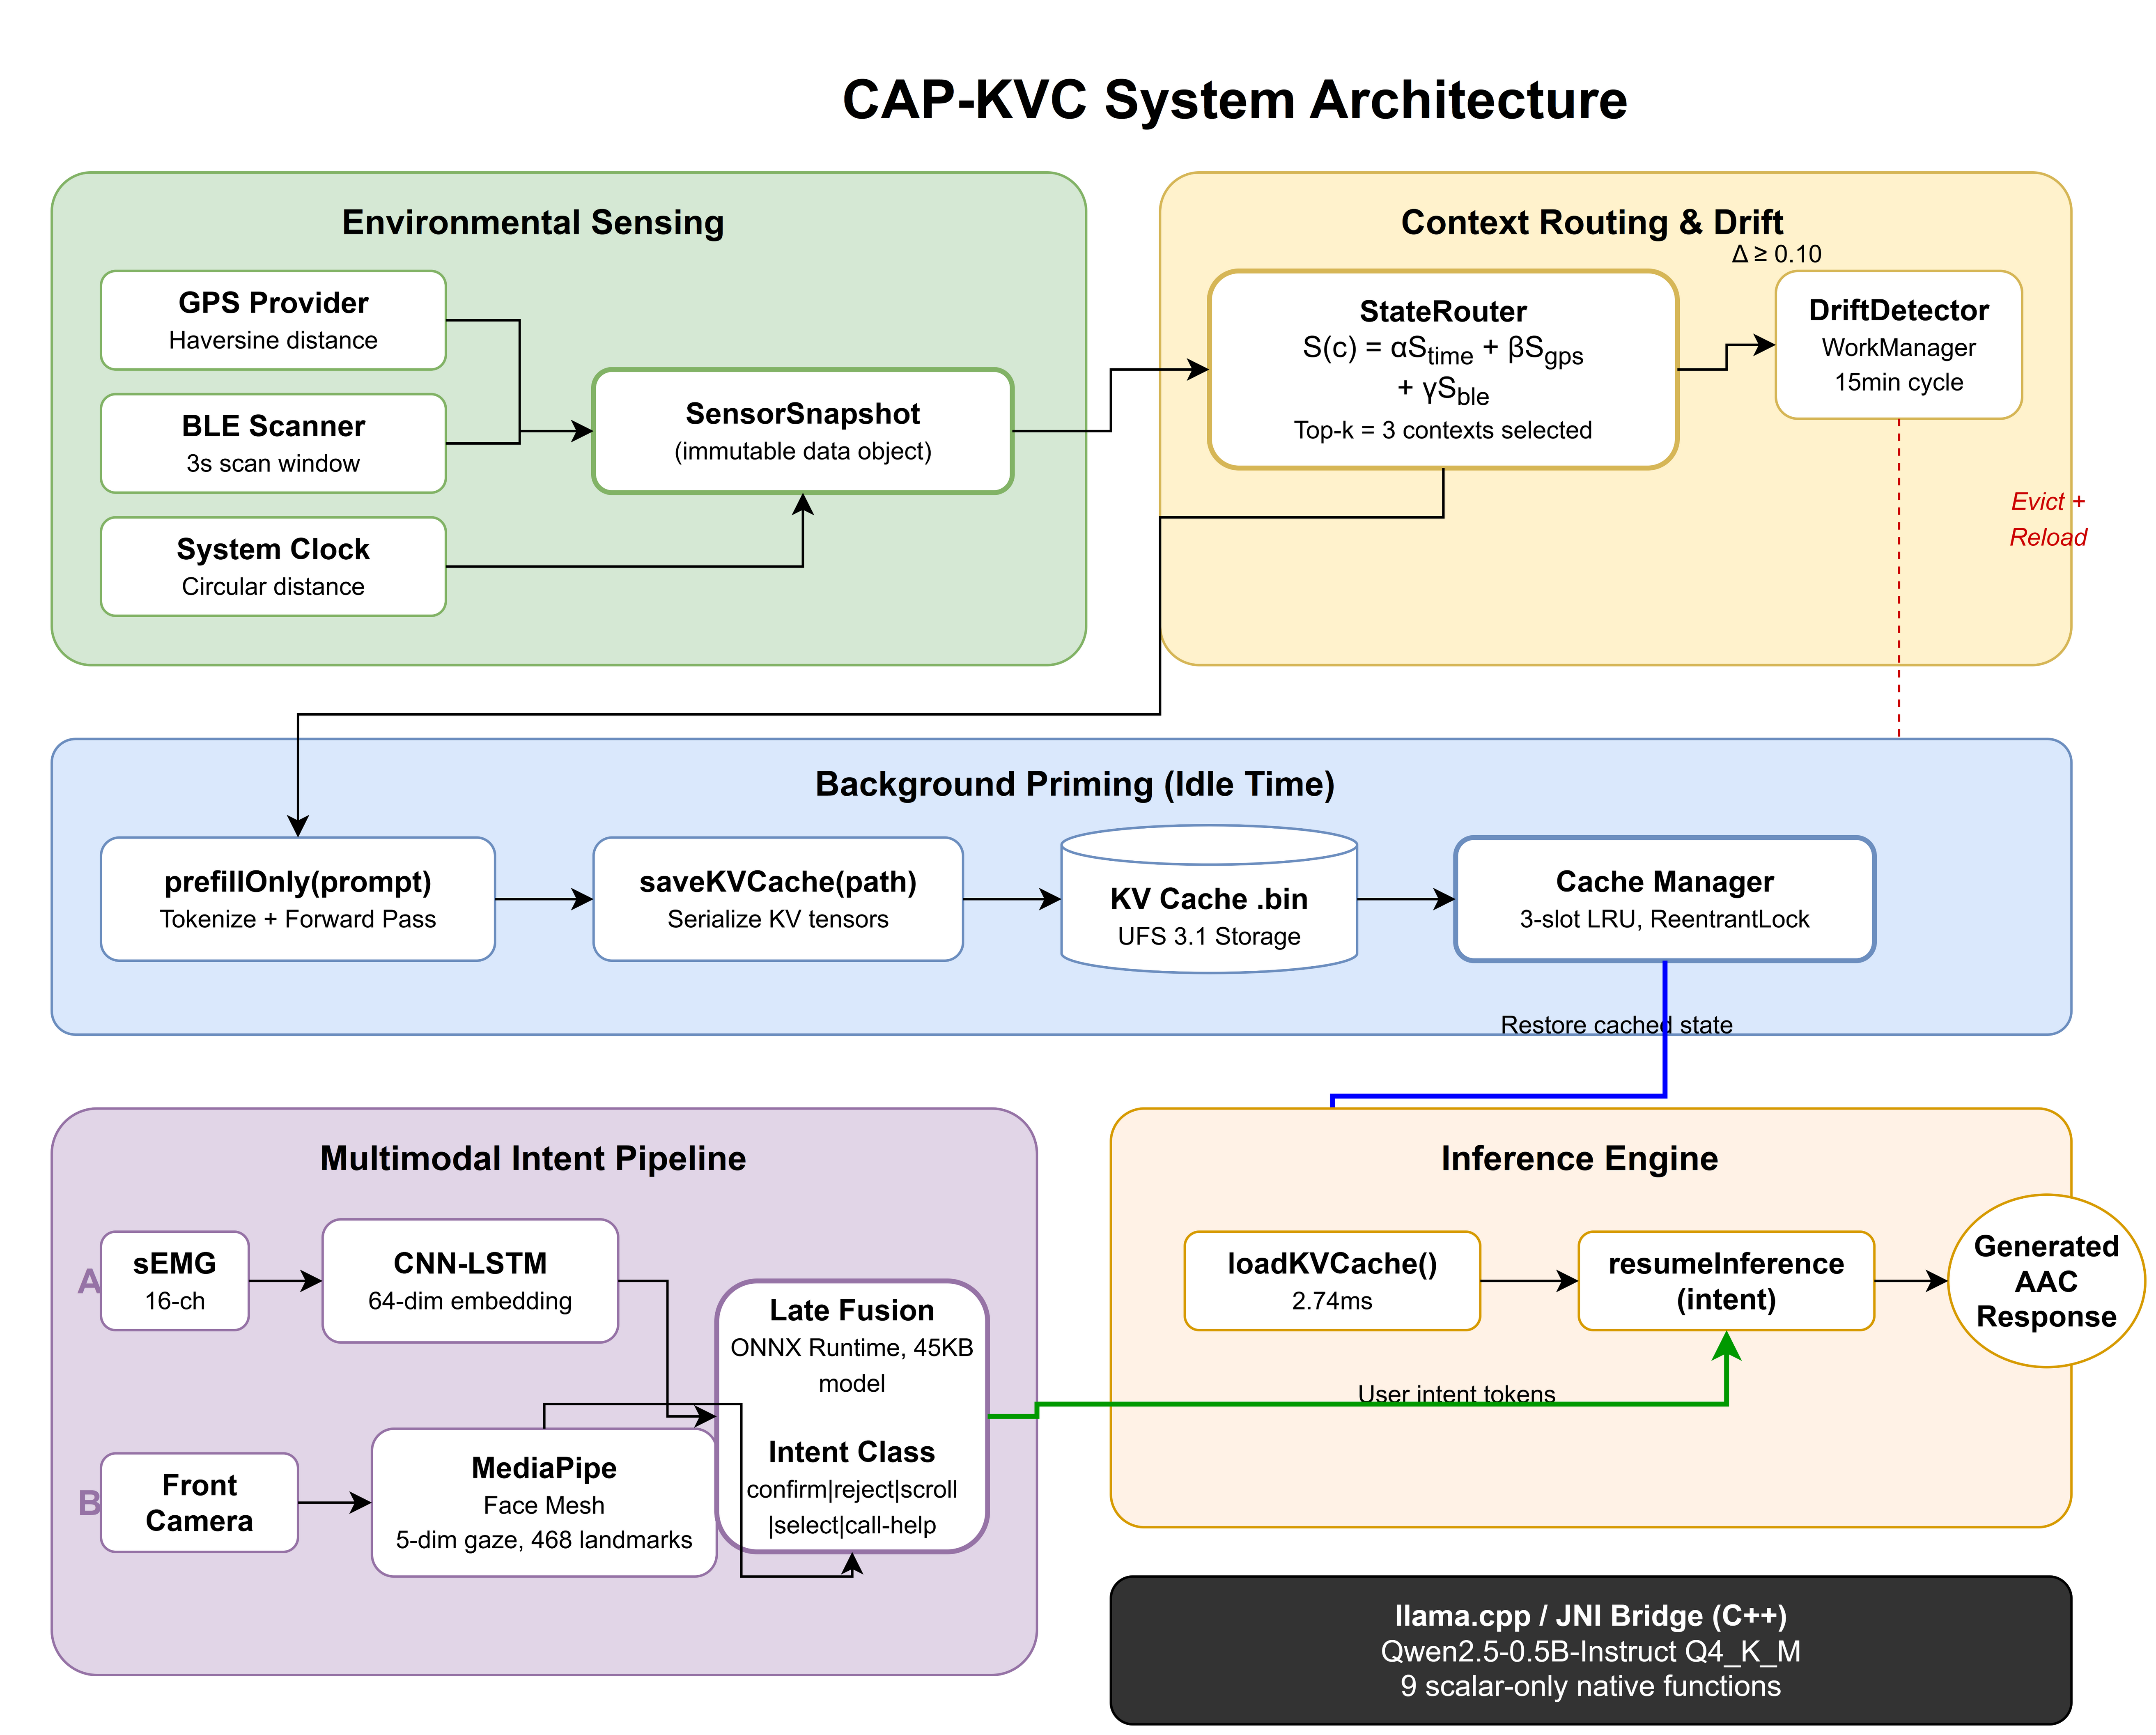
\includegraphics[width=\textwidth]{system_architecture_new.png}
\caption{CAP-KVC system architecture. Environmental sensors (blue) feed a deterministic scoring function that selects contexts for background priming (green). The multimodal intent pipeline (purple) combines sEMG and gaze inputs via late fusion. At inference time (orange), the pre-computed KV cache is restored and only intent tokens are processed by the llama.cpp/JNI backend. A periodic drift detector re-evaluates context relevance with hysteresis gating ($\Delta \geq 0.10$).}
\label{fig:architecture}
\end{figure*}

\subsection{Problem Formulation}
\label{sec:problem}

Consider a user $u$ operating an AAC device in a physical environment characterized by temporal, spatial, and proximity signals. Let $C = \{c_1, c_2, \ldots, c_M\}$ denote a finite set of pre-configured semantic contexts, each associated with a textual system prompt $p_i$ of length $N_i$ tokens. In conventional retrieval-augmented generation (RAG) pipelines, the system prompt $p_i$ is concatenated with the user's intent tokens and submitted to the language model at inference time, incurring an $O(N_i)$ prefill cost that directly adds to user-perceived latency.

CAP-KVC reformulates this as a scheduling problem: given a prediction of the user's most likely context $\hat{c}$ based on environmental signals, execute the prefill of $p_{\hat{c}}$ during idle periods and persist the resulting key-value (KV) cache tensors to persistent storage. At inference time, the system restores the pre-computed KV cache and appends only the user's intent tokens, reducing the inference-time cost from a prompt-length-dependent prefill to a cache restoration operation whose cost is independent of the original prompt length $N_i$.

\subsection{System Execution Lifecycle}
\label{sec:lifecycle}

The system operates through a five-stage pipeline, where the first three stages execute asynchronously during background idle periods and the final two stages execute at user-interaction time:

\begin{enumerate}
    \item \textbf{Sensor Acquisition.} The system concurrently polls available hardware sensors---GPS, Bluetooth Low Energy (BLE), and the system clock---to construct an immutable \texttt{SensorSnapshot} representing the user's current environmental state.

    \item \textbf{Deterministic Context Routing.} The snapshot is evaluated by a \texttt{StateRouter} against all registered semantic contexts using a convex scoring function (Section~\ref{sec:scoring}). The top-$k$ highest-scoring contexts are selected for cache residency, where $k$ is bounded by a device-specific RAM constraint (Section~\ref{sec:residency}).

    \item \textbf{Background Cache Priming.} For each selected context not already resident in memory, the system executes a background prefill of its system prompt through the language model, serializes the resulting KV cache tensors to persistent storage, and registers the context as resident.

    \item \textbf{Resident Inference.} Upon user interaction, the pre-computed KV cache for the predicted context is restored from storage into native memory. The user's intent tokens are then appended and decoded, bypassing the context prefill entirely.

    \item \textbf{Drift Correction.} An asynchronous background daemon periodically re-evaluates environmental scores to detect changes in the user's physical context and triggers cache replacement when a new context scores sufficiently higher than the weakest resident context (Section~\ref{sec:drift}).
\end{enumerate}

\subsection{Multimodal Intent Classification}
\label{sec:fusion}

User intent is derived from two complementary input modalities, fused to produce a single classification decision that is then formatted as a textual prompt for the language model.

\subsubsection{Surface Electromyography (sEMG)}
A facial sEMG wearable provides 16-channel signals sampled continuously. Raw signals are segmented into fixed-length windows and processed by a CNN-LSTM classifier that extracts a 64-dimensional embedding vector. The CNN block applies three sequential Conv1d--BatchNorm--ReLU--MaxPool layers for temporal feature extraction, followed by a two-layer LSTM for temporal context modeling. The final hidden state is projected to a 64-dimensional space and L2-normalized to produce the EMG embedding.

\subsubsection{Gaze Tracking}
A front-facing camera feeds a MediaPipe Face Mesh model~\cite{mediapipe} that extracts 468 facial landmarks at frame rate. From these, the system computes a 5-dimensional gaze feature vector from the displacement between the nose tip (landmark 4) and the eye center (midpoint of landmarks 33 and 362):

\begin{equation}
\mathbf{g} = [d_x,\; d_y,\; |d_x|,\; |d_y|,\; \sqrt{d_x^2 + d_y^2}]
\label{eq:gaze_vector}
\end{equation}

\noindent where $d_x$ and $d_y$ are the horizontal and vertical displacements in normalized image coordinates. This vector captures both directional and magnitude information while remaining invariant to face scale. A dwell-based finite state machine maps sustained gaze fixation (exceeding 400ms on a target region) to one of five discrete AAC intent classes: \emph{confirm}, \emph{reject}, \emph{scroll}, \emph{select}, and \emph{call-help}.

\subsubsection{Late Fusion Architecture}
The EMG embedding $\mathbf{e} \in \mathbb{R}^{64}$ and the gaze vector $\mathbf{g} \in \mathbb{R}^{5}$ are fused through a late fusion architecture. The gaze vector is first projected to a 64-dimensional space via a two-layer MLP, then concatenated with the EMG embedding to produce a 128-dimensional joint representation. A final two-layer classifier maps this to 5-class intent logits:

\begin{equation}
\hat{y} = \text{MLP}_{64 \rightarrow 5}\big(\text{ReLU}\big(\text{MLP}_{128 \rightarrow 64}([\mathbf{e};\; \text{proj}(\mathbf{g})])\big)\big)
\label{eq:late_fusion}
\end{equation}

Late fusion was selected over a cross-attention alternative based on a pre-specified decision criterion: cross-attention must exceed late fusion F1 by more than 3\% (absolute) to justify its additional computational and parameter overhead. The ablation results (Section~\ref{sec:results_fusion}) did not meet this threshold.

\subsection{Deterministic Context Scoring}
\label{sec:scoring}

We employ a deterministic, closed-form scoring function rather than a learned predictor to ensure bounded CPU and battery consumption during background polling. A semantic context $c_i$ is scored against the current sensor snapshot as a convex combination of three environmental similarity scores:

\begin{equation}
S(c_i) = \alpha \cdot S_{\text{time}} + \beta \cdot S_{\text{gps}} + \gamma \cdot S_{\text{ble}}
\label{eq:scoring}
\end{equation}

\noindent where $\alpha + \beta + \gamma = 1$. The weights are derived from dynamic reliability estimates of each sensor signal (Section~\ref{sec:scoring_weights}).

\subsubsection{Temporal Scoring}
The temporal similarity $S_{\text{time}}$ applies a Gaussian kernel to the circular distance between the current time and the context's expected activation time:

\begin{equation}
S_{\text{time}} = \exp\!\left(-\frac{d_{\text{circ}}(t, t_i)^2}{2\sigma^2}\right)
\label{eq:time_score}
\end{equation}

\noindent where $d_{\text{circ}}$ handles the 24-hour wraparound and $\sigma = 2.0$ hours accommodates typical schedule variability.

\subsubsection{Spatial Scoring}
The spatial similarity $S_{\text{gps}}$ applies an exponential decay to the Haversine great-circle distance between the current GPS coordinates and the context's anchor location:

\begin{equation}
S_{\text{gps}} = \exp(-\lambda \cdot d_{\text{haversine}})
\label{eq:gps_score}
\end{equation}

\noindent with $\lambda = 0.1$~km (decay constant), establishing a contextual boundary of approximately 100~meters. At $d = 100$~m, the score decays to $\approx 0.37$; at $d = 1$~km, it falls to near zero.

\subsubsection{BLE Proximity Scoring}
The BLE similarity $S_{\text{ble}}$ evaluates the overlap between currently detected Bluetooth devices and a context's registered device topology, with RSSI values mapped through a sigmoid function.

\subsubsection{Dynamic Reliability Normalization}
\label{sec:scoring_weights}
The weights $\alpha$, $\beta$, and $\gamma$ are computed dynamically from raw sensor reliability estimates rather than being statically configured. Time maintains a fixed baseline weight $w_t = 0.4$, guaranteeing that the normalization denominator $w_t + w_g + w_b$ is always positive even when both GPS and BLE are unavailable. GPS reliability $w_g$ decays exponentially with reported accuracy ($w_g = \exp(-a / 50.0)$ where $a$ is the accuracy in meters), reflecting the degradation of location precision in indoor environments. BLE reliability $w_b$ is computed from the mean sigmoid-transformed RSSI of detected devices, centered at $-70$~dBm. If GPS is unavailable ($w_g = 0$) or no BLE devices are detected ($w_b = 0$), the corresponding weight is zero and the remaining weights are renormalized to preserve the convex property $\alpha + \beta + \gamma = 1$. The value $w_t = 0.4$ was selected as an engineering heuristic to ensure meaningful temporal scoring under all sensor configurations; no systematic sensitivity analysis was performed. Contexts scoring below a dead-state threshold of 0.01 are excluded from routing consideration.

\subsection{KV Cache Residency Management}
\label{sec:residency}

The system maintains at most $k$ KV cache states simultaneously resident in native memory, where $k$ is configured based on the target device's available RAM budget ($k = 3$ in the current deployment). KV cache states are mapped to native sequence slots managed by the underlying inference engine.

When a new context requires loading and all slots are occupied, the least-recently-used (LRU) state is evicted. Eviction is protected by a reference-counting mechanism: a state undergoing active inference holds a reference that blocks eviction until inference completes. The eviction loop waits for the reference count to drain to zero before releasing the native slot.

\subsection{Asynchronous Drift Detection}
\label{sec:drift}

Environmental sensors predict physical location but cannot detect whether the conversation topic has diverged from the cached context. A periodic background daemon (executing every 15 minutes via the Android WorkManager API) re-evaluates context scores using a lightweight sensor snapshot and compares them against currently resident states.

To prevent cache thrashing under noisy sensor conditions, state replacements are gated by a hysteresis margin: a candidate context must exceed the weakest resident state's score by at least $\Delta = 0.10$ before a cache swap is authorized. This prevents oscillatory eviction-reload cycles that would impose unnecessary I/O and prefill costs.

A separate offline characterization study evaluates the sensitivity of \emph{semantic} topic-shift detection---using Sentence-BERT centroid distances on annotated DailyDialog conversations~\cite{dailydialog}---to the sliding window size $k$ used for centroid smoothing (Section~\ref{sec:results_drift}). This offline study is distinct from the deployed \texttt{DriftDetector}, which operates on sensor-score deltas rather than semantic embeddings. The offline ablation characterizes detection sensitivity as a function of $k$ on available annotated data; the deployed system's behavior is governed by the hysteresis margin $\Delta$ described above.

\subsection{Inference Fallback}
\label{sec:fallback}

If a user triggers an intent before the background daemon has successfully pre-loaded any relevant context (a ``cold miss''), the system employs a two-tier fallback pipeline. Tier~1 executes an immediate in-memory lookup of pre-configured generic responses and presents the result via text-to-speech output, maintaining immediate conversational responsiveness. Tier~2 initiates an asynchronous standard RAG prefill on the inference backend, allowing subsequent user intents to be upgraded to contextual inference once the prefill completes.

% ===========================================================================
% IV. IMPLEMENTATION
% ===========================================================================
\section{Implementation}
\label{sec:implementation}

\subsection{Platform and Runtime}
\label{sec:platform}

AACBridge targets \texttt{arm64-v8a} devices running Android~12+. The inference backend builds on \texttt{llama.cpp}~\cite{llamacpp}, using Qwen2.5-0.5B-Instruct~\cite{qwen25} quantized to Q4\_K\_M via GGUF. Pre-compiled native libraries ship inside the APK. The Kotlin layer communicates with C++ through JNI; all dependency injection is manual (no Hilt/Dagger/Koin) to minimize startup latency.

\subsection{JNI Boundary Contract}
\label{sec:jni}

The JNI layer exposes nine native functions in a single C++ source file (\texttt{llama\_jni.cpp}, 801 lines): eight application-facing plus one lifecycle cleanup (\texttt{release}). A strict constraint governs this boundary: \textbf{all arguments and return values are JNI scalar types} (\texttt{jstring}, \texttt{jint}, \texttt{jboolean}). No Java objects, arrays, or callbacks cross the boundary, eliminating JNI global references and GC root pinning.

The functions fall into three groups: \emph{lifecycle} (\texttt{initializeBackend}, \texttt{initializeModel}, \texttt{release}); \emph{KV cache operations} (\texttt{saveKVCache}, \texttt{loadKVCache}, \texttt{clearKVCache}); and \emph{inference} (\texttt{runInference}, \texttt{prefillOnly}, \texttt{resumeInference}). The distinction between \texttt{runInference} and \texttt{resumeInference} is critical: the former clears session history and processes from position zero, while the latter preserves the loaded token history and appends at position $n_{\text{past}}$, preventing position-ID collisions that would corrupt the attention computation.

\subsection{Concurrency Model}
\label{sec:concurrency}

The C++ backend maintains shared global state: a \texttt{llama\_context} pointer and a \texttt{session\_tokens} vector for KV cache consistency. A single \texttt{ReentrantLock} (the ``engine lock'') guards all JNI call sequences that depend on consistent session state. The lock is held across both \texttt{loadKVCache} and \texttt{resumeInference} within a single acquisition, since releasing between calls would let another thread mutate \texttt{session\_tokens}. Separate per-state Kotlin coroutine \texttt{Mutex} instances protect cache residency metadata without blocking unrelated operations.

\subsection{KV Cache Priming Lifecycle}
\label{sec:priming}

Context priming executes three phases per semantic state: (1)~\emph{prefill}---the engine lock is acquired and \texttt{prefillOnly(prompt)} populates the native KV cache without entering the generation loop; (2)~\emph{serialize}---while still holding the lock, \texttt{saveKVCache(tmpPath, 0)} writes KV tensors to a temporary file (slot~0 is mandatory since \texttt{prefillOnly} decodes into slot~0 via \texttt{llama\_batch\_get\_one}); (3)~\emph{atomic commit}---after releasing the lock, the temporary file is atomically renamed to the final \texttt{.bin} path, leveraging ext4's atomic \texttt{rename()}. A model-readiness gate (\texttt{AtomicBoolean}) prevents priming before native context initialization.

\subsection{KV Cache Residency and Eviction}
\label{sec:eviction}

The cache manager maintains $k = 3$ native sequence slots as a concurrent queue. When all slots are occupied, the least-recently-accessed state is evicted: the victim is marked inactive, the manager polls until its reference count drains to zero (10ms delay to avoid busy-spinning), and the slot is returned to the pool. Reusing a slot via \texttt{loadKVCache} implicitly overwrites prior KV contents after clearing via \texttt{llama\_memory\_seq\_rm}.

\subsection{Sensor Integration}
\label{sec:sensors}

Two cooperating components handle background sensing. \textbf{ActiveSweep} is a coroutine-based collector that concurrently acquires GPS (\texttt{getLastKnownLocation}) and BLE topology (3000ms \texttt{BluetoothLeScanner} window), combining both into a \texttt{SensorSnapshot}. \textbf{DriftDetector} is a \texttt{CoroutineWorker} polling every 15 minutes via WorkManager; it uses a BLE-blind snapshot to conserve battery, relying on GPS and time signals---methodologically valid because both candidate and resident states are scored against the same BLE-blind data.

A \texttt{BroadcastReceiver} for \texttt{BOOT\_COMPLETED} and \texttt{MY\_PACKAGE\_REPLACED} ensures cache population after boot or update using the \texttt{goAsync()} pattern.

\textbf{Sensing cost.} GPS uses a cached fix; BLE performs a bounded 3-second scan. The primary energy cost is background KV cache priming (one full inference per cache state), which occurs at most once per context transition during idle/charging periods.

\subsection{Fusion Model Deployment}
\label{sec:fusion_deploy}

The late fusion model is exported to ONNX and bundled as \texttt{gaze\_emg\_fusion.onnx} (45,459~bytes). On-device inference uses ONNX Runtime~\cite{onnxruntime} with a single-threaded CPU provider. The session is lazily initialized at application scope to avoid reloading during activity recreation.

Input tensors: EMG embedding ($1 \times 1 \times 64$, \texttt{float32}) and gaze vector ($1 \times 5$, \texttt{float32}). Output logits undergo argmax and numerically stable softmax to extract the predicted intent and confidence. If the ONNX session fails, the system falls back to the raw gaze target with zero confidence.

\subsection{Gaze Tracking}
\label{sec:gaze_impl}

Gaze tracking uses MediaPipe Face Landmarker~\cite{mediapipe} (bundled 3.7~MB \texttt{.task} file) in live-stream mode on CameraX frames. The gaze displacement vector (Equation~\ref{eq:gaze_vector}) maps to one of five screen quadrants plus center, each corresponding to an AAC intent class. A dwell-based finite state machine requires 400ms sustained fixation before emitting an intent, preventing accidental activation from saccades. The state machine runs on a single-threaded executor to guarantee sequential processing of asynchronous MediaPipe callbacks.

% ===========================================================================
% V. EXPERIMENTAL SETUP
% ===========================================================================
\section{Experimental Setup}
\label{sec:experiments}

\subsection{Hardware Platform}
\label{sec:hardware}

All on-device benchmarks were conducted on a OnePlus~11R (Snapdragon~8+~Gen~1, 8~GB LPDDR5X, UFS~3.1 storage) running Android~14. The device was configured in airplane mode with display brightness fixed at 50\% to minimize thermal and scheduling variability. No other foreground applications were active during benchmarking.

\subsection{Language Model Configuration}
\label{sec:model_config}

The language model used throughout evaluation is Qwen2.5-0.5B-Instruct~\cite{qwen25}, quantized to Q4\_K\_M (4-bit mixed precision) via \texttt{llama.cpp}'s GGUF serialization format. This model was selected as the smallest instruction-tuned model in the Qwen2.5 family capable of producing coherent, context-aware responses on mobile hardware. The native context is configured with \texttt{n\_ctx} $= 2048$ (maximum sequence length), \texttt{n\_batch} $= 512$ (batch processing size), and \texttt{n\_threads} $= 4$ (inference thread count). Greedy decoding is used for all inference trials via \texttt{llama\_sampler\_init\_greedy()}, which deterministically selects the highest-probability token at each step. The maximum generation length is 64 tokens, ensuring deterministic output sequences that minimize generation-phase variance across trials.

Table~\ref{tab:hyperparams} summarizes all configurable system parameters for reproducibility.

\begin{table}[htbp]
\centering
\caption{System hyperparameters. All values are fixed at compile time except the model path.}
\label{tab:hyperparams}
\begin{tabular}{llr}
\hline
\textbf{Component} & \textbf{Parameter} & \textbf{Value} \\
\hline
\multirow{4}{*}{LLM Engine} & \texttt{n\_ctx} (max sequence) & 2048 \\
 & \texttt{n\_batch} (batch size) & 512 \\
 & \texttt{n\_threads} & 4 \\
 & Max generation tokens & 64 \\
\hline
\multirow{3}{*}{Scoring} & $\alpha$ (time baseline weight) & 0.4 \\
 & $\beta, \gamma$ (GPS, BLE) & dynamic \\
 & Dead-state threshold & 0.01 \\
\hline
\multirow{2}{*}{Drift} & Hysteresis margin $\Delta$ & 0.10 \\
 & Poll interval & 15 min \\
\hline
\multirow{2}{*}{Cache} & Max active KV states & 3 \\
 & BLE scan window & 3000 ms \\
\hline
\multirow{2}{*}{Benchmark} & Warmup trials & 2 \\
 & Measured trials & 30 \\
\hline
\end{tabular}
\end{table}

\subsection{Benchmark Conditions}
\label{sec:conditions}

The latency evaluation compares three pipeline configurations:

\begin{enumerate}
    \item \textbf{ZERO\_CONTEXT}: The language model receives only the user intent tokens (``\texttt{User: I need water\textbackslash nAssistant:}'') with no environmental context. This establishes the hardware floor for inference latency on the target SoC.

    \item \textbf{RAG\_INLINE}: The full context prompt is concatenated with the user intent and submitted as a single string to \texttt{runInference()}, triggering a complete $O(N)$ token prefill at inference time. This represents the standard retrieval-augmented generation approach. Evaluated at four prompt-length tiers: $N \in \{50, 100, 200, 500\}$ approximate tokens.

    \item \textbf{CAP\_KVC}: A pre-computed KV cache is restored from persistent storage via \texttt{loadKVCache()}, followed by \texttt{resumeInference()} with intent-only tokens. The latency reported includes both the cache restoration time and the subsequent generation time.
\end{enumerate}

The CAP\_KVC condition was evaluated using cache files primed from the base context prompts ($\sim$50 tokens). The N-scaling comparison therefore compares RAG\_INLINE at increasing context lengths against CAP\_KVC at a fixed cache size. This is by design: the CAP\_KVC inference-time cost does not depend on the original context length under the evaluated configuration because the prefill was amortized during background priming. The cache restoration cost is dominated by file I/O (proportional to file size), not by attention computation.

\textbf{Important limitation:} Because the CAP\_KVC cache states were derived from $\sim$50-token context prompts, comparisons against RAG\_INLINE conditions with substantially longer contexts (e.g., $N \approx 500$) characterize \emph{inference-time amortization behavior} rather than response quality under equivalent context richness. The speedup ratios quantify the latency advantage of cache restoration over repeated prefill, not the semantic equivalence of the generated responses.

\subsection{Measurement Methodology}
\label{sec:measurement}

Each benchmark condition executes 32 sequential trials: 2~warmup trials (discarded) followed by 30~measured trials. The warmup phase absorbs JIT compilation of Kotlin/ART code paths and initial thermal settling. All measurements are wall-clock latency captured via \texttt{System.nanoTime()} at the Kotlin layer, wrapping the complete JNI call sequence.

\textbf{Prefill isolation via native instrumentation.} To decompose end-to-end latency into its constituent phases, \texttt{std::chrono::high\_resolution\_clock} timestamps are inserted immediately before and after each \texttt{llama\_decode()} call within both \texttt{runInference} and \texttt{resumeInference}. This isolates the prefill phase---the single \texttt{llama\_decode()} call that processes all prompt tokens through the transformer---from the subsequent autoregressive generation loop. The instrumentation also records the generation-phase duration (from sampler initialization through the final generated token) and emits both timings, along with prompt and generated token counts, via \texttt{\_\_android\_log\_print}. 

On the Android NDK libc++ runtime, \texttt{std::chrono::high\_resolution\_clock} maps directly to the monotonic \texttt{std::chrono::steady\_clock}, which is backed by the kernel's \texttt{CLOCK\_MONOTONIC} clock source. This prevents duration calculations from being corrupted by system NTP synchronization or manual clock adjustments. The overhead of the clock read call is $\approx 10$--50~ns (leveraging the vDSO-accelerated kernel interface), which is negligible relative to the millisecond-scale model inference. JNI boundaries, string copies, and log serialization calls occur strictly outside the timed regions.

For the CAP\_KVC condition, the benchmark instruments three sub-components separately: \texttt{cache\_load\_ms} (the \texttt{loadKVCache} call, measured at the Kotlin layer), \texttt{prefill\_ms} (the intent-only \texttt{llama\_decode} within \texttt{resumeInference}, measured at the native layer), and \texttt{gen\_ms} (the generation loop, measured at the native layer). Both Kotlin-layer and native-layer measurements are captured under the same engine lock acquisition to prevent interleaving.

Results are emitted as structured CSV lines via Android's \texttt{Log.i()} facility and extracted post-run via \texttt{adb logcat}. To mitigate the risk of packet drops or transient buffer overflows in Android's logcat ring buffer, the post-run extraction script matches JNI timing entries to Kotlin bench entries by strict proximity and asserts alignment of trial indices and token counts. Any mismatch or incomplete sequence aborts the parser to ensure data integrity; the 180 trials reported here were fully verified and aligned.

\subsection{Pre-Benchmark Validation}
\label{sec:validation}

Before executing the benchmark suite, a semantic validation pass confirms that the three pipeline configurations produce qualitatively distinct outputs. A diagnostic prompt (``\texttt{What should I have for breakfast and is my morning medication due?}'') is submitted under each condition, and the generated text is logged for manual inspection. This validates that:

\begin{itemize}
    \item ZERO\_CONTEXT produces a generic response lacking environmental specificity.
    \item RAG\_INLINE produces a response reflecting the \texttt{home\_morning} context (breakfast, medication).
    \item CAP\_KVC produces a similarly context-aware response, confirming that KV cache restoration successfully preserved the contextual attention patterns.
\end{itemize}

The benchmark suite is aborted if the KV cache load fails during validation, preventing the collection of meaningless data.

\subsection{Memory Profiling}
\label{sec:memory_profiling}

Native heap memory usage is measured using Android's \texttt{dumpsys meminfo} command at two states: (1)~after model initialization with zero KV cache states loaded, and (2)~after loading three KV cache states into native sequence slots. The delta represents the marginal memory cost of the predictive caching system.

\subsection{Fusion Model Evaluation}
\label{sec:fusion_eval}

The multimodal fusion model is evaluated through a controlled ablation study comparing two architectures:

\begin{itemize}
    \item \textbf{Cross-Attention}: A single-head cross-attention module ($d = 64$) where the EMG embedding serves as the query and the projected gaze vector serves as key and value.
    \item \textbf{Late Fusion}: Concatenation of the 64-dimensional EMG embedding and the 64-dimensional projected gaze vector, followed by a two-layer MLP classifier.
\end{itemize}

Both architectures are trained on a synthetic dataset of 2000 paired EMG-gaze samples (60\% train, 20\% validation, 20\% test) drawn from a synthetic data generator that pairs random EMG embeddings with corresponding gaze vectors. The pre-specified decision criterion requires that the cross-attention model exceed the late fusion model's macro F1 score by more than 3~percentage points (absolute) to justify deployment of the more complex architecture.

\textbf{Limitation:} The fusion training data is synthetically generated and does not represent real paired EMG-gaze recordings from AAC users. The reported accuracy and F1 scores characterize the model's capacity to learn the fusion mapping under controlled conditions, not its expected clinical accuracy. This is explicitly acknowledged as a limitation of the current evaluation.

\subsection{EMG Classifier Evaluation}
\label{sec:emg_eval}

The CNN-LSTM EMG classifier is trained on a subset of the NinaPro~DB5 dataset~\cite{ninapro} using a leave-one-subject-out (LOSO) protocol: subjects~1--9 for training and subject~10 for validation. Training uses the Adam optimizer with learning rate $10^{-3}$, cosine annealing schedule, class-weighted cross-entropy loss, and gradient clipping at norm~1.0. The model is trained for up to 50~epochs with early stopping based on validation accuracy.

The EMG classifier operates as an embedding extractor for the downstream fusion model. Its standalone classification accuracy on the held-out subject is reported separately from the fusion accuracy to avoid conflation.

\subsection{Drift Detection Ablation}
\label{sec:drift_eval}

The sensitivity of conversation-level drift detection to the sliding window size $k$ is evaluated offline on the DailyDialog dataset~\cite{dailydialog}. Each conversation is annotated with ground-truth topic shift indices. For each $k \in \{1, 2, 3, 4, 5\}$, the system computes the centroid embedding of the most recent $k$ turns using Sentence-BERT (\texttt{all-MiniLM-L6-v2}~\cite{minilm}), and predicts a topic shift when the cosine similarity between the anchor embedding and the centroid falls below a threshold $\theta = 0.15$. Precision, recall, and F1 are computed for each $k$. The MiniLM model is used solely for this offline ablation analysis and is not part of the deployed Android runtime; the on-device drift detector operates on router score deltas rather than semantic embeddings.

\textbf{Limitation:} DailyDialog is a general-purpose dialogue corpus that differs substantially from AAC communication patterns in terms of turn length, vocabulary, and topic variability. The k-ablation results characterize the detector's behavior on available annotated data rather than providing direct evidence of clinical effectiveness.

% ===========================================================================
% VI. RESULTS
% ===========================================================================
\section{Results}
\label{sec:results}

\subsection{End-to-End Inference Latency (RQ1)}
\label{sec:results_latency}

Table~\ref{tab:latency} summarizes the end-to-end inference latency across all benchmark conditions ($n = 30$ measured trials per condition, 180 total measurements).

\begin{table}[htbp]
\centering
\caption{Inference latency decomposition (ms) across pipeline conditions. Prefill isolates the \texttt{llama\_decode()} forward pass; generation covers the autoregressive sampling loop. Both are measured via native-side \texttt{std::chrono} instrumentation. CAP\_KVC total includes cache restoration, prefill, and generation. All values: OnePlus~11R, Qwen2.5-0.5B-Instruct Q4\_K\_M, greedy sampling, max 64~output tokens, $n = 30$ trials.}
\label{tab:latency}
\resizebox{\columnwidth}{!}{%
\begin{tabular}{lrrrrr}
\hline
\textbf{Condition} & \textbf{E2E (ms)} & \textbf{Prefill (ms)} & \textbf{Gen (ms)} & \textbf{E2E $\sigma$} & \textbf{Tokens} \\
\hline
ZERO\_CONTEXT       & 3823.78 & 274.79  & 3544.58  & 569.76  & 9  \\
RAG ($N\!\approx\!50$)  & 6547.13 & 2021.46 & 4508.53  & 8392.58 & 52 \\
RAG ($N\!\approx\!100$) & 7900.92 & 3015.09 & 4877.95  & 3857.18 & 89 \\
RAG ($N\!\approx\!200$) & 12122.30 & 6673.53 & 5439.96 & 2740.12 & 206 \\
RAG ($N\!\approx\!500$) & 19408.89 & 14001.46 & 5390.76 & 2113.04 & 439 \\
\hline
CAP\_KVC (cache load)       & 2.74  & ---  & ---  & 1.35 & --- \\
CAP\_KVC (inference)        & 4571.97 & 343.35 & 4226.74  & 373.65 & 9  \\
CAP\_KVC (total)            & 4574.70 & ---    & ---      & 373.49 & ---  \\
\hline
\end{tabular}%
}
\end{table}

Fig.~\ref{fig:latency_comparison} visualizes these results, and Fig.~\ref{fig:latency_breakdown} provides a detailed breakdown showing the stacked composition of CAP-KVC latency.

\begin{figure}[htbp]
\centering
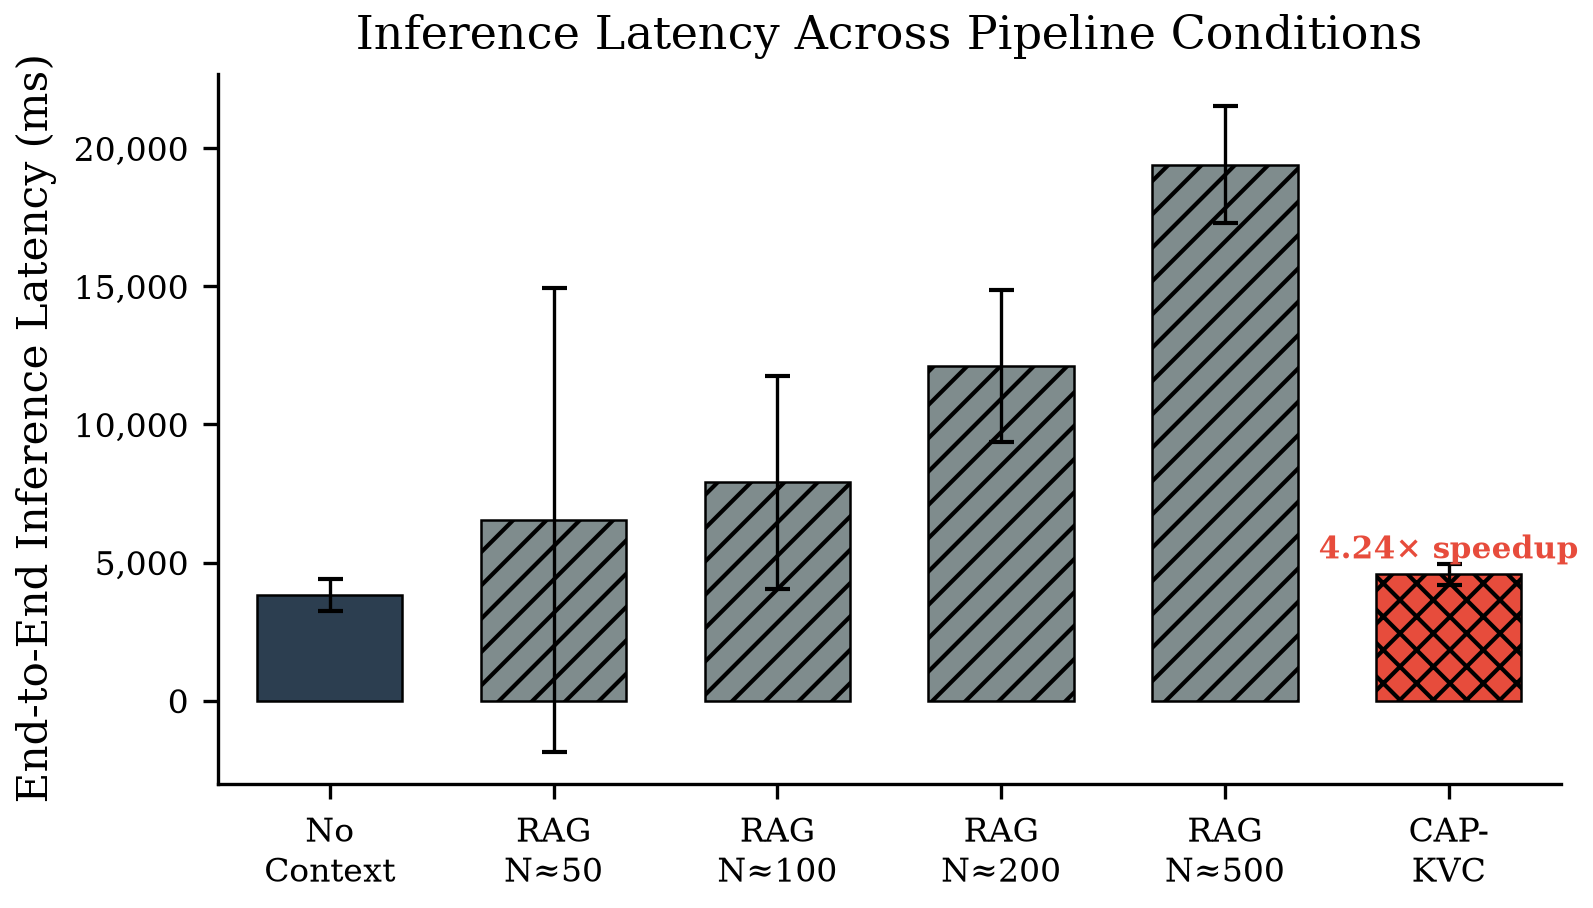
\includegraphics[width=\columnwidth]{latency_comparison_new.png}
\caption{End-to-end inference latency across pipeline conditions ($n = 30$ trials each). Error bars indicate one standard deviation. CAP-KVC achieves a 4.24$\times$ end-to-end speedup relative to RAG\_INLINE at $N \approx 500$.}
\label{fig:latency_comparison}
\end{figure}

\begin{figure}[htbp]
\centering
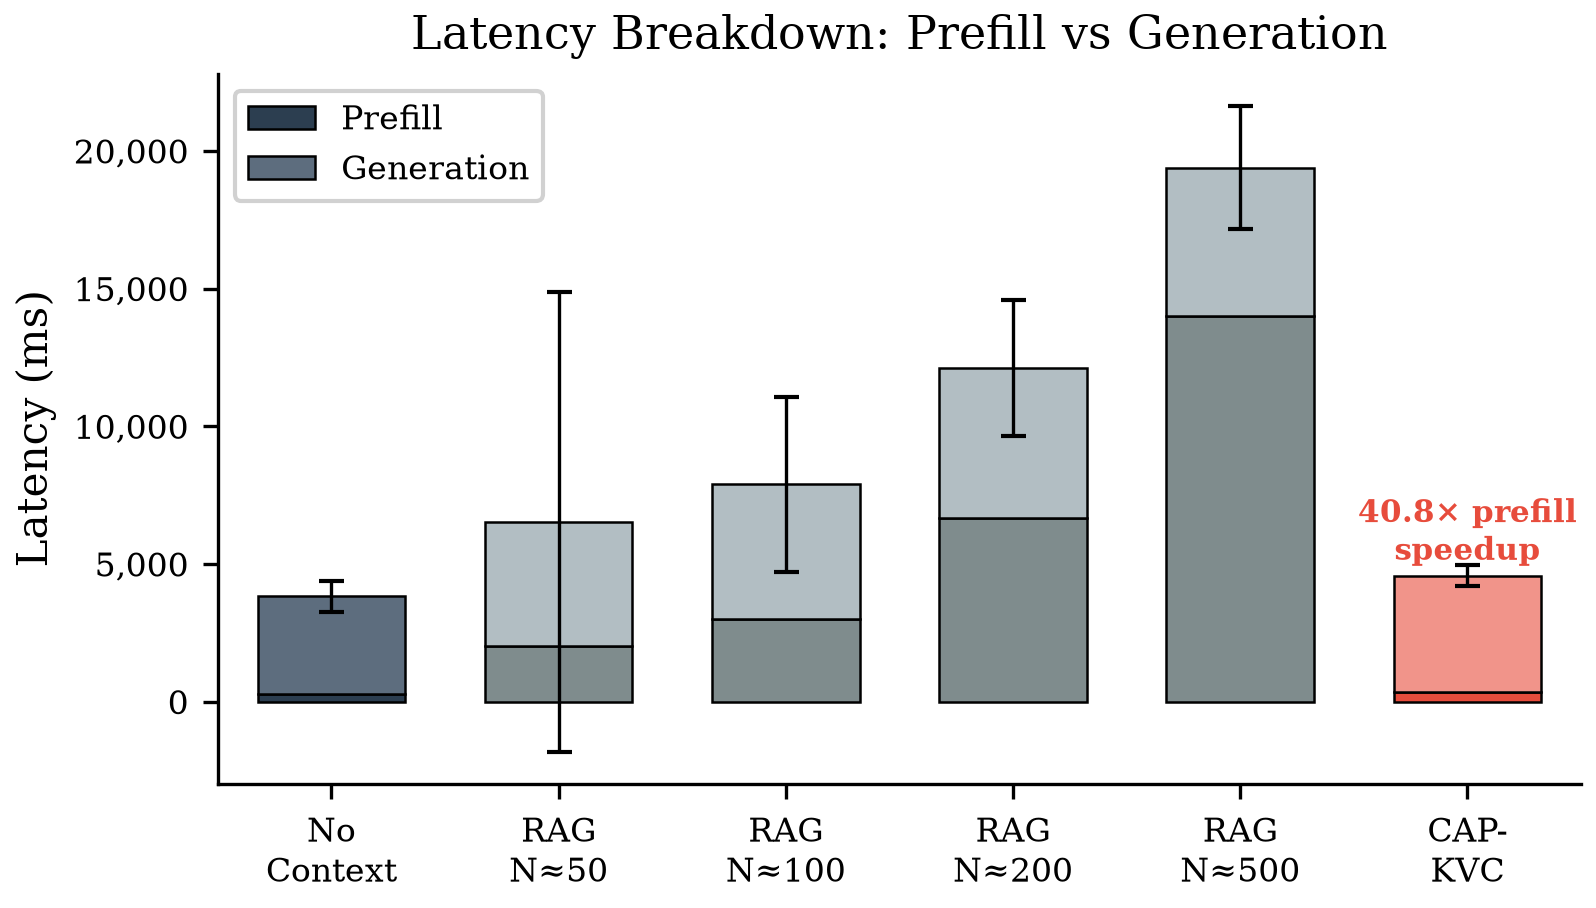
\includegraphics[width=\columnwidth]{latency_breakdown_new.png}
\caption{Latency breakdown across pipeline conditions. Native-side \texttt{std::chrono} instrumentation decomposes each trial into prefill (dark) and generation (light) phases. RAG\_INLINE prefill scales linearly with context length (274~ms at $N\!=\!9$ to 14001~ms at $N\!=\!439$ tokens), whereas CAP\_KVC prefill is 343~ms regardless of cached context size, achieving a 40.78$\times$ prefill-specific speedup. Error bars: one standard deviation ($n = 30$).}
\label{fig:latency_breakdown}
\end{figure}

\textbf{Cache restoration is negligible.} The mean cache load time is 2.74~ms ($\sigma = 1.35$~ms), representing less than 0.1\% of the total CAP\_KVC latency. This duration measures the complete Kotlin-side \texttt{loadKVCache()} round trip, including JNI marshalling, native file I/O, and KV tensor deserialization. The restoration is dominated by hardware I/O and memory copy rather than computational processing.

\textbf{CAP\_KVC avoids context-proportional prefill.} The native-side prefill decomposition (Table~\ref{tab:latency}) confirms that RAG\_INLINE prefill scales linearly with prompt length: from 2021~ms at $N \approx 52$ tokens to 14001~ms at $N \approx 439$ tokens, a 6.93$\times$ increase. In contrast, the CAP\_KVC prefill cost is 343.35~ms ($\sigma = 45.00$~ms) for 9 intent-only tokens, regardless of the cached context size. This represents a \textbf{40.78$\times$ prefill speedup} relative to RAG\_INLINE at $N \approx 500$.

\textbf{Speedup relative to RAG\_INLINE.} End-to-end, CAP\_KVC achieves a total latency of 4574.70~ms versus RAG\_INLINE's 19408.89~ms at $N \approx 500$, an end-to-end speedup of 4.24$\times$. At $N \approx 50$, the mean end-to-end speedup is 1.43$\times$ (6547.13 / 4574.70), though this end-to-end difference is not statistically significant ($p = 0.209$) due to high variance in the RAG\_INLINE generation phase; the prefill-specific speedup at $N \approx 50$ remains statistically significant ($p = 0.011$). The prefill decomposition reveals that the end-to-end speedup is heavily masked by the generation phase, which is comparable across conditions ($\sim$3500--5400~ms).

\textbf{Statistical significance and assumptions.} Welch's two-sample $t$-tests ($\alpha = 0.05$, two-tailed) on the \emph{prefill-only} latency confirm statistical significance: CAP\_KVC versus RAG\_INLINE at $N \approx 50$ ($t(29.0) = -2.71$, $p = 0.011$, Cohen's $d = 0.70$) and CAP\_KVC versus RAG\_INLINE at $N \approx 500$ ($t(29.0) = -40.42$, $p < 10^{-26}$, Cohen's $d = 10.44$). The end-to-end comparison at $N \approx 500$ is also significant ($t(30.8) = -37.86$, $p < 10^{-26}$, $d = 9.78$). 

Although Welch's $t$-test is robust to unequal variances (which are expected due to prompt-dependent prefill scaling), the extreme skewness of the underlying RAG latency distributions violates standard parametric normality assumptions. The resulting $t$-test statistics should be interpreted as general trends rather than exact probabilities. For $N \approx 50$ prefill, Cohen's $d = 0.70$ indicates a medium-to-large effect. For $N \approx 500$, $d = 10.44$ represents an overwhelming effect. Cohen's $d$ was computed using equal-sample pooled variance; we note that this value is attenuated by the high variance of the RAG condition.

\textbf{Outlier analysis.} For diagnostic purposes, Tukey's outlier criterion ($Q_3 + 3 \times \text{IQR}$) was applied to identify extreme latency anomalies. This flagged 5 outlier trials (3 in RAG@50, 1 in ZERO\_CONTEXT, 1 in CAP\_KVC) exhibiting latency substantially above the condition mean. The precise mechanism underlying these outliers---whether OS-level thermal management, background scheduler preemption, garbage collection pauses, or other system-level effects---was not independently measured during the benchmark run. No thermal telemetry, CPU frequency logs, or scheduler event traces were captured alongside the benchmark data. To ensure scientific conservatism and preserve the operational reality of edge hardware, these outliers were not removed from the statistics reported in Table~\ref{tab:latency} or the primary t-test calculations.

\textbf{Generation-phase analysis.} The generation-phase duration varies across conditions: ZERO\_CONTEXT 3544~ms (58 tokens), RAG\_INLINE@50 4508~ms (64 tokens), RAG\_INLINE@500 5390~ms (64 tokens), and CAP\_KVC 4226~ms (64 tokens). The variation in generation time is consistent with two factors: (1)~differences in per-token attention computation cost when the KV cache contains different numbers of entries, and (2)~system-level effects associated with sustained mobile execution over a 29-minute benchmark session (the benchmark captured no thermal telemetry or CPU frequency data to distinguish specific mechanisms). Critically, because prefill and generation are now decomposed, these generation-phase differences do not confound the prefill speedup measurement.

\subsection{Multimodal Fusion Ablation (RQ3)}
\label{sec:results_fusion}

Table~\ref{tab:fusion} presents the ablation comparison between the two candidate fusion architectures, evaluated on the synthetic test set (400 samples).

\begin{table}[htbp]
\centering
\caption{Fusion architecture ablation results. Values from \texttt{fusion\_ablation.csv}. Latency is per-sample CPU inference time.}
\label{tab:fusion}
\begin{tabular}{lcccc}
\hline
\textbf{Architecture} & \textbf{Accuracy} & \textbf{F1 (Macro)} & \textbf{Precision} & \textbf{Recall} \\
\hline
Cross-Attention & 0.9467 & 0.9437 & 0.9459 & 0.9450 \\
Late Fusion     & \textbf{0.9967} & \textbf{0.9963} & 0.9956 & 0.9972 \\
\hline
\end{tabular}
\end{table}

Late fusion achieves a macro F1 of 0.9963 compared to 0.9437 for cross-attention, a difference of 5.26~percentage points. Because the cross-attention model \emph{underperforms} the simpler architecture rather than exceeding it, the pre-specified 3\% superiority threshold is not met, and the late fusion model is selected for deployment. The automated decision logic writes the winning architecture identifier to a file (\texttt{winner.txt}), and the corresponding model checkpoint (\texttt{late\_fusion\_best.pth}, 48~KB) is exported to ONNX format and bundled in the application assets. Fig.~\ref{fig:fusion_ablation} visualizes the comparison.

\begin{figure}[htbp]
\centering
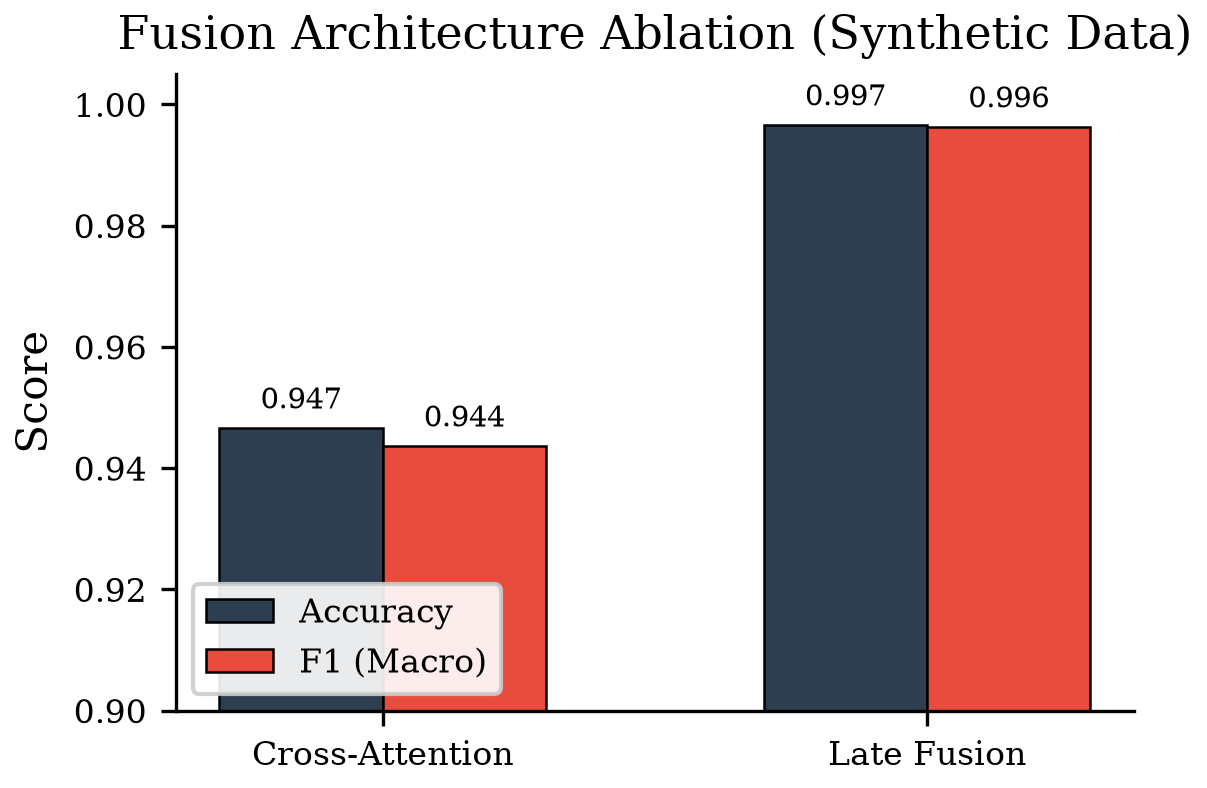
\includegraphics[width=\columnwidth]{fusion_ablation_new.png}
\caption{Fusion architecture ablation on synthetic test data (400 samples). Late fusion exceeds cross-attention in both accuracy and F1.}
\label{fig:fusion_ablation}
\end{figure}

\textbf{Synthetic data caveat.} The training and evaluation data are synthetically generated, pairing random EMG embeddings with gaze vectors. The high accuracy reflects the model's capacity to learn the intended fusion mapping under controlled conditions and validates that the late fusion architecture can successfully combine heterogeneous embedding spaces of differing dimensionality ($\mathbb{R}^{64}$ and $\mathbb{R}^{5}$). These numbers should not be interpreted as predictions of clinical intent-recognition accuracy on real paired EMG-gaze recordings from AAC users, where sensor noise, electrode placement variability, and user-specific physiological differences would substantially affect performance.

\subsection{EMG Classifier Performance}
\label{sec:results_emg}

The standalone CNN-LSTM EMG classifier, evaluated on the held-out subject (LOSO protocol, subject~10), achieves a test accuracy of 42.4\% with a macro F1 of 0.37. Table~\ref{tab:emg} shows the per-class breakdown.

\begin{table}[htbp]
\centering
\caption{EMG standalone classification report (held-out subject). Values from \texttt{classification\_report.txt}.}
\label{tab:emg}
\begin{tabular}{lcccc}
\hline
\textbf{Class} & \textbf{Precision} & \textbf{Recall} & \textbf{F1} & \textbf{Support} \\
\hline
confirm   & 0.25 & 0.11 & 0.15 & 18 \\
reject    & 0.00 & 0.00 & 0.00 & 18 \\
scroll    & 0.42 & 0.72 & 0.53 & 18 \\
select    & 0.77 & 0.50 & 0.61 & 20 \\
call-help & 0.45 & 0.78 & 0.57 & 18 \\
\hline
\textbf{Macro avg} & 0.38 & 0.42 & 0.37 & 92 \\
\hline
\end{tabular}
\end{table}

The low standalone accuracy is expected under cross-subject evaluation, where inter-subject variability in facial EMG patterns is a well-documented challenge~\cite{ninapro}. The \emph{reject} class is entirely unrecognized (0\% recall), and the model exhibits a strong bias toward the \emph{scroll} and \emph{call-help} classes, as visible in the confusion matrix (Fig.~\ref{fig:emg_confusion}). The training curves (Fig.~\ref{fig:training_curves}) show clear overfitting: training accuracy reaches approximately 80\% by epoch~35 while validation accuracy plateaus near 40\%, with the best checkpoint selected at epoch~8 (validation accuracy $\approx$~47\%).

\begin{figure}[htbp]
\centering
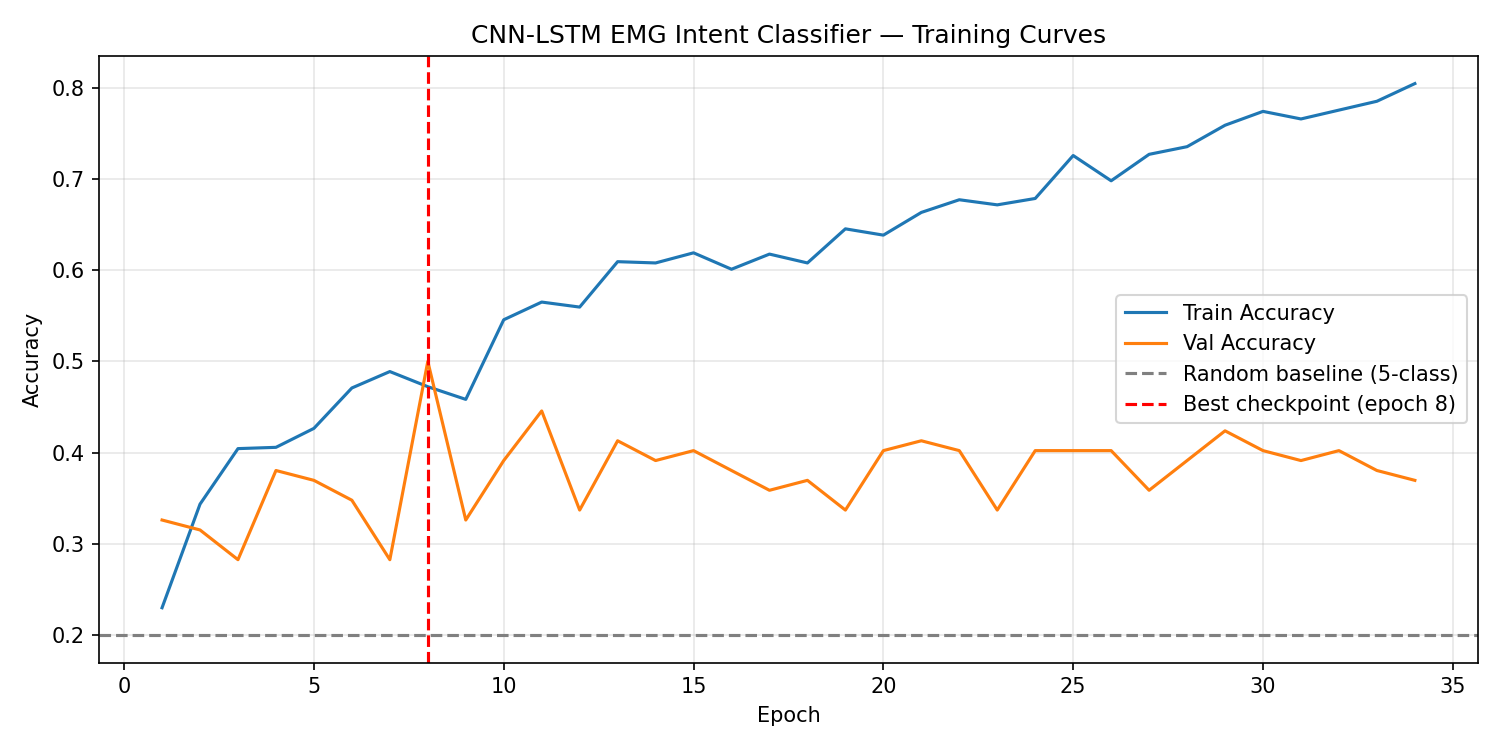
\includegraphics[width=\columnwidth]{training_curves.png}
\caption{CNN-LSTM EMG classifier training and validation accuracy over 35 epochs. The red dashed line marks the best checkpoint at epoch~8. The gray dashed line indicates the 5-class random baseline (20\%).}
\label{fig:training_curves}
\end{figure}

\begin{figure}[htbp]
\centering
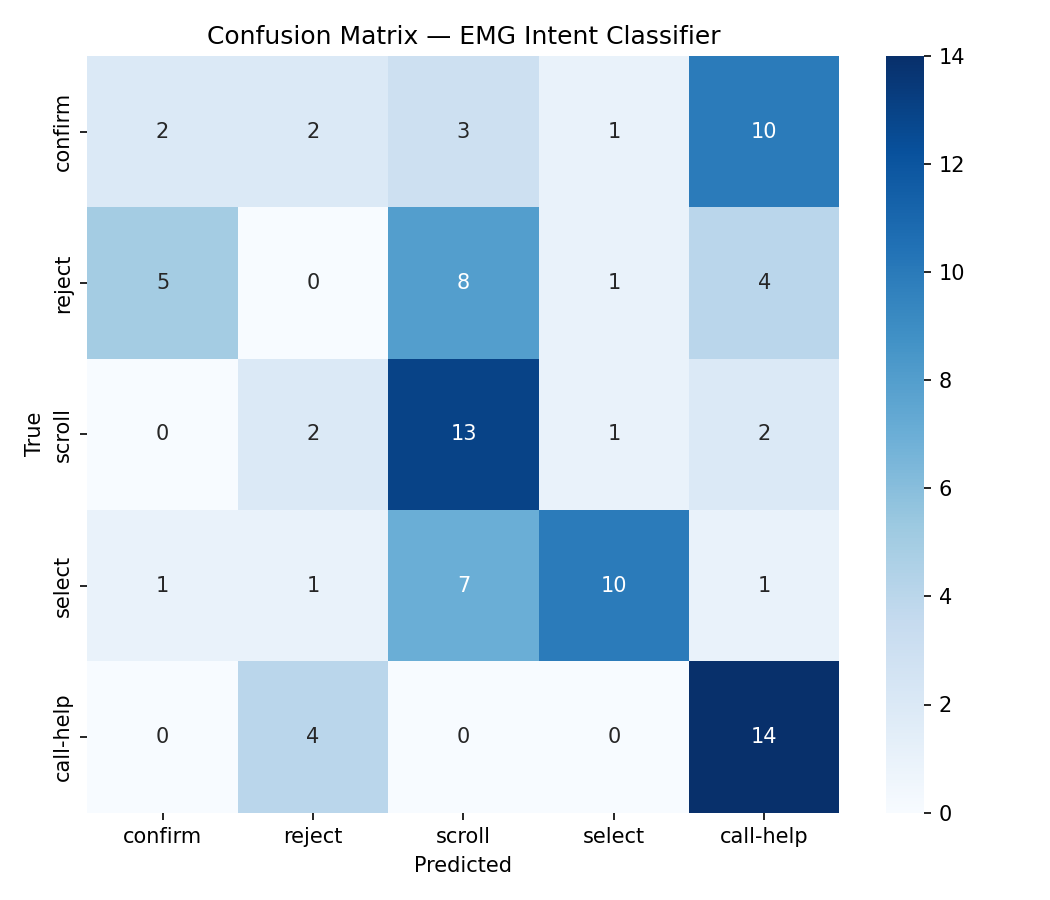
\includegraphics[width=\columnwidth]{emg_confusion_matrix.png}
\caption{Confusion matrix for the EMG standalone classifier on the held-out subject. Strong \emph{call-help} and \emph{scroll} diagonal entries contrast with near-zero \emph{confirm} and \emph{reject} performance.}
\label{fig:emg_confusion}
\end{figure}

These results demonstrate that the standalone EMG classifier does not achieve sufficient accuracy for deployment as a primary intent recognizer under cross-subject conditions. The multimodal fusion approach compensates by combining the EMG embedding with gaze tracking, achieving higher classification performance on the synthetic evaluation set (Section~\ref{sec:results_fusion}). However, no gaze-only baseline was evaluated, so the claim that fusion improves upon both unimodal channels independently is \textbf{not supported} by the current experimental design. The on-device CNN-LSTM inference latency is 1.98~ms (mean, $\sigma = 1.12$~ms, $n = 200$ trials), indicating that embedding extraction is feasible within real-time constraints.

\subsection{Memory Budget (RQ2)}
\label{sec:results_memory}

Table~\ref{tab:memory} reports native heap usage measured via \texttt{dumpsys meminfo} at two operating points.

\begin{table}[htbp]
\centering
\caption{Native heap memory usage (KB) from \texttt{dumpsys meminfo}. Delta represents the marginal cost of loading three KV cache states.}
\label{tab:memory}
\begin{tabular}{lrr}
\hline
\textbf{State} & \textbf{Native Heap (KB)} & \textbf{Total PSS (KB)} \\
\hline
Idle (0 states)     & 18,856  & 623,488 \\
Loaded (3 states)   & 140,420 & 612,940 \\
\hline
\textbf{Delta}      & +121,564 ($\approx$118.7~MB) & --- \\
\hline
\end{tabular}
\end{table}

The three-state KV cache residency adds approximately 118.7~MB of native heap (121,564~KiB $\div$ 1024). The total PSS (proportional set size) decreases slightly between states due to measurement variability in shared memory attribution. The native heap growth is consistent with three copies of the model's KV cache tensors ($\sim$40~MB per state for a 0.5B-parameter model at Q4\_K\_M quantization). Fig.~\ref{fig:memory_budget} visualizes the two operating points.

\begin{figure}[htbp]
\centering
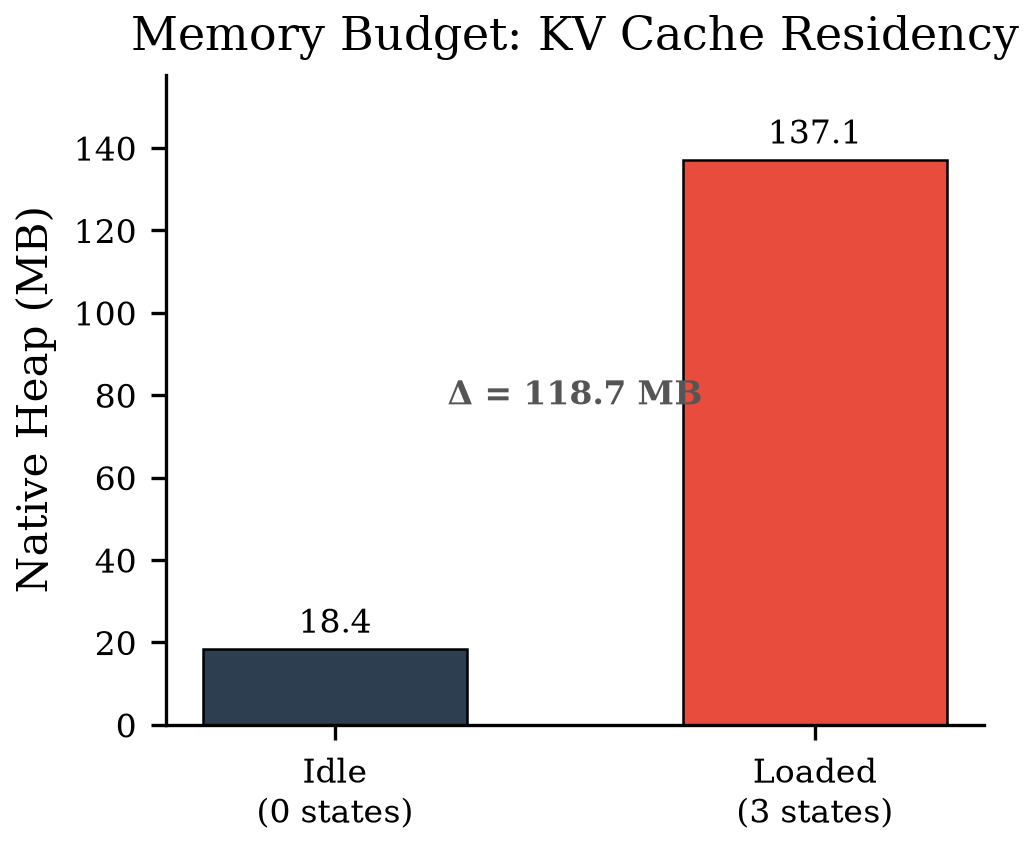
\includegraphics[width=\columnwidth]{memory_budget_new.png}
\caption{Native heap memory usage at idle (0 KV states) and with 3 KV cache states loaded. The delta of 118.7~MB represents the marginal cost of predictive caching.}
\label{fig:memory_budget}
\end{figure}

\subsection{Drift Detection Ablation}
\label{sec:results_drift}

Table~\ref{tab:drift} presents the k-ablation results for the offline semantic drift detection characterization on annotated DailyDialog conversations ($\theta = 0.15$). This evaluation uses Sentence-BERT centroid distances~\cite{minilm} to detect topic shifts in text transcripts and is methodologically distinct from the deployed \texttt{DriftDetector}, which operates on environmental sensor-score deltas (Section~\ref{sec:drift}).

\begin{table}[htbp]
\centering
\caption{Drift detection F1 as a function of sliding window size $k$, evaluated on DailyDialog with $\theta = 0.15$. $n_{\text{true}}$ and $n_{\text{pred}}$ denote the number of ground-truth and predicted shift points, respectively.}
\label{tab:drift}
\begin{tabular}{ccccccc}
\hline
$k$ & $\theta$ & Precision & Recall & F1 & $n_{\text{true}}$ & $n_{\text{pred}}$ \\
\hline
1 & 0.15 & 0.367 & 0.367 & \textbf{0.367} & 150 & 150 \\
2 & 0.15 & 0.341 & 0.313 & 0.326 & 150 & 138 \\
3 & 0.15 & 0.137 & 0.107 & 0.120 & 150 & 117 \\
4 & 0.15 & 0.071 & 0.040 & 0.051 & 150 & 84 \\
5 & 0.15 & 0.039 & 0.013 & 0.020 & 150 & 52 \\
\hline
\end{tabular}
\end{table}

The highest F1 (0.367) is achieved at $k = 1$, with performance degrading monotonically as the window size increases (Fig.~\ref{fig:drift_kablation}). This indicates that the centroid smoothing introduced by larger $k$ values reduces sensitivity to genuine topic shifts under the selected threshold. However, the absolute F1 values are low across all $k$ (ranging from 0.367 to 0.020), reflecting both the inherent difficulty of unsupervised topic-shift detection and the substantial mismatch between DailyDialog's multi-turn conversational dynamics and the sparse, short-turn interactions typical of AAC usage.

\textbf{Deployment rationale for $k = 3$.} The deployed \texttt{DriftDetector} uses $k = 3$ for its sensor-score smoothing window. The DailyDialog ablation operates on a different detection mechanism (Sentence-BERT centroid distances) and cannot directly inform the deployed sensor-score threshold. The value $k = 3$ was retained as an engineering smoothing heuristic: in the mobile environment, sensor score sequences are noisier than annotated dialogue transcripts, and a larger window provides stability against transient fluctuations. The choice should be understood as a conservative design decision rather than an empirically validated parameter.

\begin{figure}[htbp]
\centering
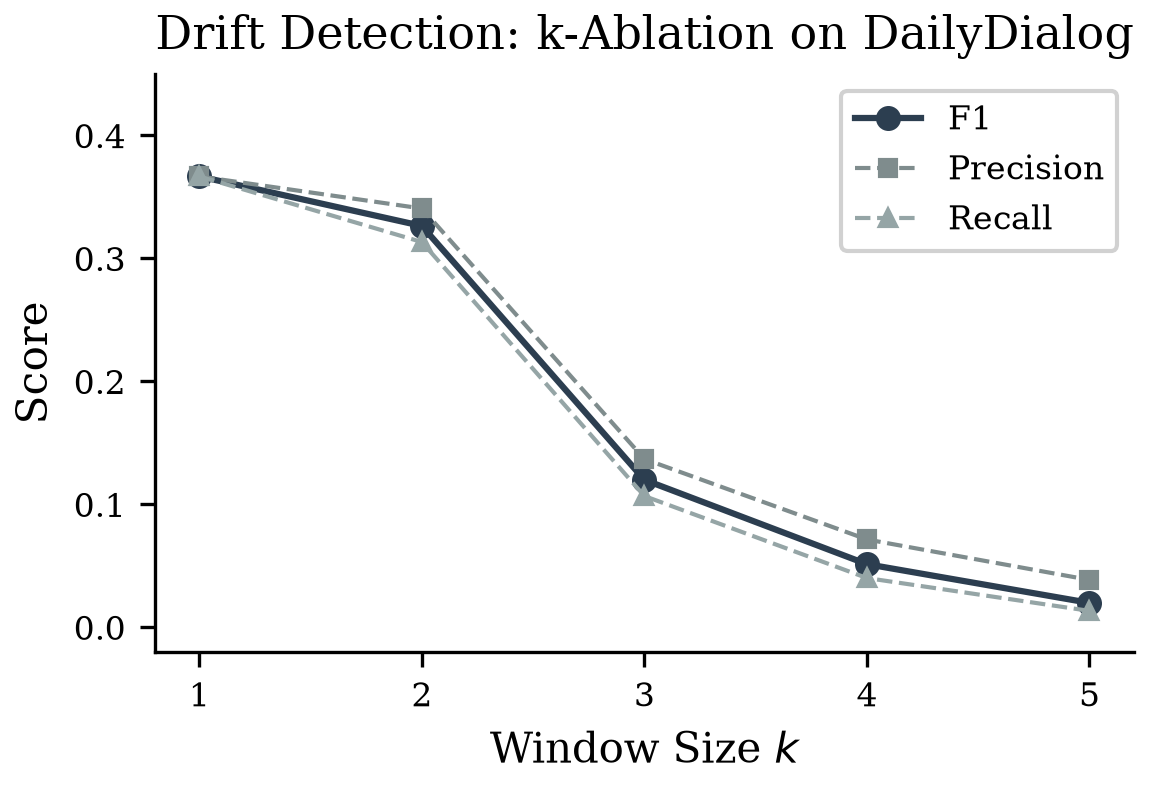
\includegraphics[width=\columnwidth]{drift_k_ablation_new.png}
\caption{Drift detection precision, recall, and F1 as a function of sliding window size $k$ on DailyDialog ($\theta = 0.15$). Performance degrades monotonically with increasing $k$.}
\label{fig:drift_kablation}
\end{figure}

\subsection{Summary of Key Findings}
\label{sec:results_summary}

The experimental results support the following conclusions:

\begin{enumerate}
    \item CAP-KVC achieves a 40.78$\times$ prefill-specific speedup at $N \approx 500$ tokens (343~ms vs.\ 14001~ms), confirmed by native-side \texttt{std::chrono} instrumentation. The end-to-end speedup is 4.24$\times$ (4574~ms vs.\ 19408~ms), with the generation phase ($\sim$4000--5400~ms) accounting for the difference between prefill and end-to-end ratios. Cache restoration is 2.74~ms (negligible).

    \item The late fusion architecture achieves a macro F1 of 0.9963 on synthetic evaluation data, exceeding cross-attention (F1~=~0.9437) while requiring fewer parameters and lower inference latency, supporting the pre-specified selection criterion.

    \item The standalone EMG classifier achieves 42.4\% accuracy under cross-subject evaluation, motivating multimodal fusion as a necessary complement rather than a standalone solution.

    \item The three-state KV cache residency requires approximately 118.7~MB of additional native heap, a feasible budget on modern mobile devices with 8~GB RAM.

    \item Drift detection on DailyDialog yields a maximum F1 of 0.367 ($k = 1$), suggesting that the chosen threshold ($\theta = 0.15$) and evaluation corpus may require further calibration for clinical AAC deployment.
\end{enumerate}

% ===========================================================================
% VII. CONCLUSION
% ===========================================================================
\section{Conclusion}
\label{sec:conclusion}

CAP-KVC amortizes context prefill costs for on-device language model inference by predicting environmental context from sensor signals and pre-computing KV cache states during idle periods. Native-side prefill decomposition on a OnePlus~11R with Qwen2.5-0.5B-Instruct (Q4\_K\_M) confirms a 40.78$\times$ prefill-specific speedup at $N \approx 500$ tokens (343~ms vs.\ 14001~ms) and a 4.24$\times$ end-to-end reduction (4574~ms vs.\ 19408~ms), with cache restoration completing in 2.74~ms.

The Android implementation uses a scalar-only JNI boundary (9~native functions), reentrant-lock concurrency, and a bounded cache manager operating within 118.7~MB native heap for three simultaneous states. A proof-of-concept multimodal intent layer achieves macro F1 = 0.9963 on synthetic data through late fusion of sEMG and gaze inputs; clinical validation remains necessary.

The core insight is that sensor-driven predictive caching can eliminate prompt-length-dependent prefill latency on edge devices. The approach generalizes beyond AAC: any mobile application where a language model processes recurring environmental contexts can exploit idle-time cache priming.

\subsection{Limitations}

Several limitations constrain the generalizability of these results and should be addressed in future evaluations:

\begin{enumerate}
    \item \textbf{Single-device, limited-sample evaluation.} All benchmarks were conducted on a single device (OnePlus~11R, Snapdragon~8+~Gen~1) with $n = 30$ measured trials per condition. Latency characteristics, thermal behavior, and memory budgets may differ on other mobile SoCs, and the moderate sample size limits the precision of variance estimates.

    \item \textbf{Single model.} Only Qwen2.5-0.5B-Instruct (Q4\_K\_M) was evaluated. The relationship between CAP-KVC speedup and model size, quantization level, or architecture family has not been characterized.

    \item \textbf{Synthetic fusion data.} The fusion model was trained and evaluated on synthetically generated EMG-gaze pairs. The reported macro F1 of 0.9963 reflects model capacity under controlled conditions and does not predict clinical accuracy. No gaze-only unimodal baseline was evaluated.

    \item \textbf{Latency metric scope.} The prefill timing (Table~\ref{tab:latency}) measures the single \texttt{llama\_decode()} batch-decode call via native-side \texttt{std::chrono} instrumentation. Tokenization and batch construction overhead (estimated $< 1$~ms for prompts up to 500 tokens) are excluded. Generation-phase duration varies across conditions due to differing KV cache sizes affecting per-token attention cost and uncharacterized system-level effects during the 29-minute benchmark session. No thermal telemetry, CPU frequency logs, or OS scheduler traces were captured during the benchmark run, so the specific mechanisms underlying generation-phase variance cannot be attributed. Because prefill and generation are decomposed independently, these generation-phase differences do not confound the prefill speedup measurement.

    \item \textbf{Static context configurations.} The benchmarking uses five pre-configured semantic contexts rather than dynamically learned user profiles. A production deployment would require user-configurable contexts and longitudinal evaluation of context relevance.

    \item \textbf{No non-predictive cache baseline.} The evaluation compares CAP-KVC against inline context processing (RAG\_INLINE) and zero-context inference but does not include a static cache baseline (i.e., a fixed pre-loaded KV cache without prediction or drift detection). Such a baseline would isolate the contribution of the predictive routing and drift components from the raw benefit of cache restoration itself.

    \item \textbf{Drift detection.} The offline Sentence-BERT k-ablation yields a maximum F1 of 0.367 ($k = 1$) on DailyDialog, while the deployed sensor-score-based system uses $k = 3$. These are methodologically different detection mechanisms, and the DailyDialog results cannot directly validate the deployed sensor-score hysteresis. Both the window size ($k = 3$) and threshold ($\theta = 0.15$, $\Delta = 0.10$) are engineering heuristics.

    \item \textbf{No clinical evaluation.} The system has not been evaluated with AAC users in clinical or naturalistic settings. User satisfaction, communicative effectiveness, and caregiver acceptance remain to be assessed.

    \item \textbf{No thermal or power telemetry.} The benchmark run captured only application-level timing data via \texttt{adb logcat} filtered to the AACBridge process. No thermal sensor readings, CPU frequency logs, OS-level thermal management events, or power consumption measurements were collected during the 29-minute benchmark session. Consequently, the specific mechanisms underlying latency outliers and generation-phase variance cannot be attributed to thermal throttling versus other system-level effects.

    \item \textbf{No cache file encryption.} Serialized KV cache tensors are stored as raw binary files in the application's internal storage directory. Protection relies entirely on the Android application sandbox; no additional encryption or integrity verification is applied. In threat models involving rooted devices or physical access, cached KV tensors---which encode the semantic content of contextual prompts---could be extracted.

    \item \textbf{Battery impact not characterized.} The \texttt{ContextDaemon} foreground service (60-second sweep interval) and the \texttt{DriftDetector} periodic worker (15-minute interval via WorkManager) impose recurring sensor acquisition and, when cache states require priming, full model inference. The aggregate battery impact of these background operations has not been measured. No WakeLock, PowerManager, or battery-level gating is implemented beyond the Android system's standard WorkManager batching behavior and the daemon's \texttt{onLowMemory()} sweep cancellation. Additionally, the coroutine-based \texttt{delay()} scheduling in \texttt{ContextDaemon} does not hold a WakeLock, so sweep intervals may be deferred by Android Doze mode when the device is idle and stationary.
\end{enumerate}

Despite these limitations, the results demonstrate that predictive KV cache priming is a viable strategy for reducing context-dependent inference latency on resource-constrained mobile hardware, and that the cache restoration cost ($\sim$3~ms) is negligible relative to the generation phase.

\subsection{Artifact Availability}

The source code, benchmark scripts, and raw benchmark logs are publicly available at \url{https://github.com/omni-ar/AACBridge}.

% ===========================================================================
% REFERENCES
% ===========================================================================
\begin{thebibliography}{30}

\bibitem{beukelman2020}
D.~R. Beukelman and J.~C. Light,
``Augmentative and alternative communication: Supporting children and adults with complex communication needs,''
\emph{Paul H. Brookes Publishing}, 5th ed., 2020.

\bibitem{llamacpp}
G.~Gerganov,
``llama.cpp: LLM inference in {C/C++},''
2023. [Online]. Available: \url{https://github.com/ggerganov/llama.cpp}

\bibitem{qwen25}
A.~Yang, B.~Yang, B.~Hui, B.~Zheng, B.~Yu, \emph{et al.},
``{Qwen2.5 Technical Report},''
\emph{arXiv preprint arXiv:2412.15115}, 2024.

\bibitem{dettmers2022}
T.~Dettmers, M.~Lewis, Y.~Belkada, and L.~Zettlemoyer,
``{LLM.int8(): 8-bit matrix multiplication for transformers at scale},''
in \emph{Proc. NeurIPS}, 2022.

\bibitem{frantar2022}
E.~Frantar, S.~Ashkboos, T.~Hoefler, and D.~Alistarh,
``{GPTQ: Accurate post-training quantization for generative pre-trained transformers},''
in \emph{Proc. ICLR}, 2023.

\bibitem{mlcllm}
MLC Team,
``{MLC LLM}: Universal {LLM} deployment engine,''
2023. [Online]. Available: \url{https://github.com/mlc-ai/mlc-llm}

\bibitem{scissorhands}
Z.~Liu, A.~Desai, F.~Liao, W.~Wang, V.~Xie, Z.~Xu, A.~Kyrillidis, and A.~Shrivastava,
``Scissorhands: Exploiting the persistence of importance hypothesis for {LLM} {KV} cache compression at test time,''
in \emph{Proc. NeurIPS}, 2023.

\bibitem{h2o}
Z.~Zhang, Y.~Sheng, T.~Zhou, T.~Chen, L.~Zheng, R.~Cai, Z.~Song, Y.~Tian, C.~R\'{e}, C.~Barrett, Z.~Wang, and B.~Chen,
``{H$_2$O: Heavy-hitter oracle for efficient generative inference of large language models},''
in \emph{Proc. NeurIPS}, 2023.

\bibitem{streamingllm}
G.~Xiao, Y.~Tian, B.~Chen, S.~Han, and M.~Lewis,
``{Efficient streaming language models with attention sinks},''
\emph{arXiv preprint arXiv:2309.17453}, 2023.

\bibitem{sglang}
L.~Zheng, L.~Yin, Z.~Xie, C.~Sun, J.~Huang, C.~H.~Yu, S.~Cao, C.~Kozyrakis, I.~Stoica, J.~E.~Gonzalez, C.~W.~Barrett, and Y.~Sheng,
``{SGLang: Efficient execution of structured language model programs},''
in \emph{Proc. NeurIPS}, 2024.

\bibitem{vllm}
W.~Kwon, Z.~Li, S.~Zhuang, Y.~Sheng, L.~Zheng, C.~H.~Yu, J.~E.~Gonzalez, H.~Zhang, and I.~Stoica,
``{Efficient memory management for large language model serving with PagedAttention},''
in \emph{Proc. 29th SOSP}, 2023.

\bibitem{infinigen}
W.~Lee, J.~Lee, J.~Seo, and J.~Sim,
``{InfiniGen: Efficient generative inference of large language models with dynamic KV cache management},''
in \emph{Proc. 18th USENIX OSDI}, 2024.

\bibitem{cachegen}
Y.~Liu, H.~Li, Y.~Cheng, S.~Ray, Y.~Huang, Q.~Zhang, K.~Du, J.~Yao, S.~Lu, G.~Ananthanarayanan, M.~Maire, H.~Hoffmann, A.~Holtzman, and J.~Jiang,
``{CacheGen: KV cache compression and streaming for fast large language model serving},''
in \emph{Proc. ACM SIGCOMM}, 2024.

\bibitem{ninapro}
M.~Atzori, A.~Gijsberts, C.~Castellini, B.~Caputo, A.-G.~M.~Hager, S.~Elsig, G.~Giatsidis, F.~Bassetto, and H.~M\"{u}ller,
``{Electromyography data for non-invasive naturally-controlled robotic hand prostheses},''
\emph{Scientific Data}, vol.~1, p.~140053, 2014.

\bibitem{mediapipe}
C.~Lugaresi, J.~Tang, H.~Nash, C.~McClanahan, E.~Uboweja, M.~Hays, F.~Zhang, C.-L.~Chang, M.~G.~Yong, J.~Lee, \emph{et al.},
``{MediaPipe: A framework for building perception pipelines},''
2019. [Online]. Available: \url{https://mediapipe.dev}

\bibitem{vertanen2015}
K.~Vertanen and P.~O.~Kristensson,
``{Complementing text entry evaluations with a composition task},''
\emph{ACM Trans. Comput.-Hum. Interact.}, vol.~21, no.~5, pp.~1--33, 2015.

\bibitem{ngiam2011}
J.~Ngiam, A.~Khosla, M.~Kim, J.~Nam, H.~Lee, and A.~Y.~Ng,
``{Multimodal deep learning},''
in \emph{Proc. 28th ICML}, 2011.

\bibitem{dailydialog}
Y.~Li, H.~Su, X.~Shen, W.~Li, Z.~Cao, and S.~Niu,
``{DailyDialog: A manually labelled multi-turn dialogue dataset},''
\emph{arXiv preprint arXiv:1710.03957}, 2017.

\bibitem{minilm}
W.~Wang, F.~Wei, L.~Dong, H.~Bao, N.~Yang, and M.~Zhou,
``{MiniLM: Deep self-attention distillation for task-agnostic compression of pre-trained transformers},''
in \emph{Proc. NeurIPS}, 2020.

\bibitem{snapkv}
Y.~Li, Y.~Huang, B.~Yang, B.~Venkitesh, A.~Locatelli, H.~Ye, T.~Cai, P.~Lewis, and D.~Chen,
``{SnapKV: LLM Knows What You are Looking for Before Generation},''
\emph{arXiv preprint arXiv:2404.14469}, 2024.

\bibitem{promptcache}
I.~Gim, G.~Chen, S.-J.~Lee, N.~Sarda, A.~Khandelwal, and L.~Zhong,
``{Prompt Cache: Modular Attention Reuse for Low-Latency Inference},''
in \emph{Proc. MLSys}, 2024.

\bibitem{cacheblend}
J.~Yao, H.~Li, Y.~Liu, S.~Ray, Y.~Huang, Q.~Zhang, K.~Du, S.~Lu, G.~Ananthanarayanan, M.~Maire, H.~Hoffmann, A.~Holtzman, and J.~Jiang,
``{CacheBlend: Fast Large Language Model Serving for RAG with Cached Knowledge Fusion},''
\emph{arXiv preprint arXiv:2405.16444}, 2024.

\bibitem{powerinfer2}
Z.~Xue, Y.~Huang, S.~Du, L.~Lu, H.~Chen, J.~Wen, Y.~Zhang, X.~Li, Z.~Li, W.~Zhang, X.~Zhuang, L.~Xia, Z.~Xu, S.~Song, Y.~Xu, D.~Shu, L.~Yuan, and H.~Chen,
``{PowerInfer-2: Fast Large Language Model Inference on a Smartphone},''
\emph{arXiv preprint arXiv:2406.06282}, 2024.

\bibitem{kvquant}
C.~Hooper, S.~Kim, H.~Mohammadzadeh, M.~W.~Mahoney, Y.~S.~Shao, K.~Keutzer, and A.~Gholami,
``{KVQuant: Towards 10 Million Context Length LLM Inference with KV Cache Quantization},''
in \emph{Proc. NeurIPS}, 2024.

\bibitem{awq}
J.~Lin, J.~Tang, H.~Tang, S.~Yang, W.-M.~Chen, W.-C.~Wang, G.~Xiao, X.~Dang, C.~Gan, and S.~Han,
``{AWQ: Activation-Aware Weight Quantization for LLM Compression and Acceleration},''
in \emph{Proc. MLSys}, 2024.

\bibitem{mobilellm}
Z.~Liu, C.~Zhao, F.~Iandola, C.~Lai, Y.~Tian, I.~Fedorov, Y.~Xiong, E.~Chang, Y.~Shi, R.~Krishnamoorthi, L.~Lai, and V.~Chandra,
``{MobileLLM: Optimizing Sub-billion Parameter Language Models for On-Device Use Cases},''
in \emph{Proc. ICML}, 2024.

\bibitem{llminaflash}
K.~Alizadeh, I.~Mirzadeh, D.~Belenko, K.~Khatamifard, M.~Cho, C.~C.~Del~Mundo, M.~Rastegari, and M.~Farajtabar,
``{LLM in a Flash: Efficient Large Language Model Inference with Limited Memory},''
\emph{arXiv preprint arXiv:2312.11514}, 2023.

\bibitem{flexgen}
Y.~Sheng, L.~Zheng, B.~Yuan, Z.~Li, M.~Ryabinin, B.~Chen, P.~Liang, C.~R\'{e}, I.~Stoica, and C.~Zhang,
``{FlexGen: High-Throughput Generative Inference of Large Language Models with a Single GPU},''
in \emph{Proc. ICML}, 2023.

\bibitem{vaswani2017}
A.~Vaswani, N.~Shazeer, N.~Parmar, J.~Uszkoreit, L.~Jones, A.~N.~Gomez, {\L}.~Kaiser, and I.~Polosukhin,
``{Attention is all you need},''
in \emph{Proc. NeurIPS}, 2017.

\bibitem{onnxruntime}
ONNX Runtime Contributors,
``{ONNX Runtime},''
2021. [Online]. Available: \url{https://onnxruntime.ai}

\end{thebibliography}

\end{document}
